% MSc dissertation example file, February 2022
%
% Leave one of the documentclass lines uncommented to match your degree.
% You may remove the logo option if it causes problems.
% Do not change any other options.
% \documentclass[logo,msc,adi]{infthesis}     % Adv Design Inf
% \documentclass[logo,msc,ai]{infthesis}      % AI
% \documentclass[logo,msc,cogsci]{infthesis}  % Cognitive Sci
% \documentclass[logo,msc,cs]{infthesis}      % Computer Sci
\documentclass[logo,msc,cyber]{infthesis}   % Cyber Sec
% \documentclass[logo,msc,datasci]{infthesis} % Data Sci
% \documentclass[logo,msc,di]{infthesis}      % Design Inf
% \documentclass[logo,msc,dsti]{infthesis}    % Data Sci TI
% \documentclass[logo,msc,inf]{infthesis}     % Informatics
% \documentclass[logo,msc]{infthesis}           % degree unspecified, do not change except to add your degree
%%%%%%%%%%%%%%%%%%%%%%%%
% Understand any problems and seek approval before assuming it's ok to remove ugcheck.
\usepackage{msccheck}

% Include any packages you need below, but don't include any that change the page
% layout or style of the dissertation. By including the ugcheck package above,
% you should catch most accidental changes of page layout though.

\usepackage{listings}
\usepackage{xcolor}

\colorlet{punct}{red!60!black}
\definecolor{background}{HTML}{EEEEEE}
\definecolor{delim}{RGB}{20,105,176}
\colorlet{numb}{magenta!60!black}

\lstdefinelanguage{json}{
    basicstyle=\normalfont\ttfamily,
    numbers=left,
    numberstyle=\scriptsize,
    stepnumber=1,
    numbersep=8pt,
    showstringspaces=false,
    breaklines=true,
    frame=lines,
    backgroundcolor=\color{background},
    literate=
     *{0}{{{\color{numb}0}}}{1}
      {1}{{{\color{numb}1}}}{1}
      {2}{{{\color{numb}2}}}{1}
      {3}{{{\color{numb}3}}}{1}
      {4}{{{\color{numb}4}}}{1}
      {5}{{{\color{numb}5}}}{1}
      {6}{{{\color{numb}6}}}{1}
      {7}{{{\color{numb}7}}}{1}
      {8}{{{\color{numb}8}}}{1}
      {9}{{{\color{numb}9}}}{1}
      {:}{{{\color{punct}{:}}}}{1}
      {,}{{{\color{punct}{,}}}}{1}
      {\{}{{{\color{delim}{\{}}}}{1}
      {\}}{{{\color{delim}{\}}}}}{1}
      {[}{{{\color{delim}{[}}}}{1}
      {]}{{{\color{delim}{]}}}}{1},
}

\usepackage{microtype} % recommended, but you can remove if it causes problems

   
% Add graphicx package with pdf flag (must use pdflatex)
\usepackage[pdftex]{graphicx}  
% Better support for URLs
\usepackage{url}
% Date formating
\usepackage{datetime}

\usepackage{caption}
\usepackage{subcaption}
\usepackage{multirow}
\usepackage{pifont}

\newcommand*\rot{\multicolumn{1}{R{90}{1em}}}

\begin{document}
\begin{preliminary}

\title{Evaluating the Performance And Anonymity of Mix Networks}

\author{Erodotos Demetriou}

\date{\today}

\abstract{ Mix Networks is a means of anonymous communication that obliterates
    any link between senders and receivers by routing messages through a chain
    of nodes, also known as Mixes. The literature describes several topological
    structures - Cascade, Multi-Cascade, Stratified and Mesh - and mixing
    techniques - Time-based, Threshold Based, Pool and Continous - we can employ
    to form a Mix Network. Each configuration can independently affect the
    anonymity - measured in Entropy - and latency of a network. Recently,
    researchers developed two simulators (MiXiM and Simulator) to evaluate the
    performance and anonymity of various Mix Network arrangements. In this work,
    we compare both simulators to find out which has the potential to support
    future research. Results suggest that Piotrowska's Simulator provides
    trusted quality results. Further, we conduct a short replication study to
    reason about recent developments regarding Mix Network designs. We manage to
    partially yet accurately replicate previous research. The results are sound
    for Simulator, but this is not the case for MiXiM. Ultimately, we modify one
    of the simulators to support dynamically and statically imbalanced
    Stratified networks, reporting the impact on anonymity and latency. A
    dynamically imbalanced network assumes that Mixes might fail on each
    transmission round with a certain probability. In contrast, a statically
    imbalanced Stratified network assumes a different fixed number of Mixes per
    layer. It is essential to mention that in this work, we exclusively use
    Continuous mixing. The trials' outcome suggests that anonymity and latency
    are not affected for statically and dynamically imbalanced networks,
    especially when many users participate. Despite that, for small user bases,
    we notice a slight anonymity deviation. Configurations with fewer Mixes have
    a thin advantage in terms of Entropy. Finally, our work has introduced the
    notion of Stratified imbalanced networks. Yet we are confident that future
    developments will further extend and research imbalanced topologies assuming
    various mixing techniques. }

\maketitle

\newenvironment{ethics}
   {\begin{frontenv}{Research Ethics Approval}{\LARGE}}
   {\end{frontenv}\newpage}

\begin{ethics}
% IF ETHICS APPROVAL WAS NOT REQUIRED:
This project was planned in accordance with the Informatics Research
Ethics policy. It did not involve any aspects that required approval
from the Informatics Research Ethics committee.

\standarddeclaration
\end{ethics}


\begin{acknowledgements}
Any acknowledgements go here.
\end{acknowledgements}


\tableofcontents
\end{preliminary}


\chapter{Introduction}

The predawn of the 21st century was marked by unprecedented growth in the
information technology field, especially after the commercialisation of the
World Wide Web. Every household got plugged into the internet, and every person
could navigate through web pages, shop online, send emails and communicate with
others across the globe. During that era, the internet was a safe place
predominantly used by academics and hobbyists. However, once everyone became a
potential user, crime shifted from the analogue to the digital world.

Many hacker groups have different reasons for attacking private communication
channels, targeting personal information, such as passwords, credit card
numbers, and government emails. Hackers can be (a) cybercriminals who want to
exploit users' data for profit, (b) governments targeting private messages for
national interest or (c) security researchers challenging and enhancing systems
\cite{anderson2020security}.


Nowadays, we overcome most of the vulnerabilities related to plain-data
transfers over the wire/air using the notion of cryptography. Even though this
mechanism seems to provide adequate security, it fails to encapsulate metadata
concealment \cite{stallings2018computer}. Metadata such as the message size, the
communication duration, the message origin and destination leak information of
an encrypted, "secure" transmission. A global adversary passively eavesdropping
on every network node can statistically observe a message's sender and receiver
with a certain probability \cite{stallings2018computer}. Characteristically, the
former National Security Agency (NSA) \cite{nsa} and Central Intelligence Agency
(CIA) \cite{cia} director General Michael Hayden said that "we kill people based
on metadata" \cite{granick_2017}. Hence, researchers have been steering towards
new means of communication that respect users' privacy and improve anonymity.

Mix Networks (Mixnets) provide a solution to the metadata anonymity issue by
routing equal-sized messages through a chain of nodes (Mixes). Mixes shuffle
messages using different techniques to obliterate any link between the sender
and the receiver. 

The Mixnets pioneer David Chaum proposed Cascade networks as a tool for a
hard-to-trace electronic mail exchange system back in 1981
\cite{chaum1981untraceable}. Nevertheless, his idea did not succeed due to (a)
the high computational requirements of such a system, (b) the significant
network latency and (c) the lack of quality implementations\cite{ben2021mixim}.
Soon, researchers realised the potential of Mixnets and their applications to
many domains. Such applications include remailers \cite{remailers,mixmaster,
danezis2003mixminion}, instant messaging apps\cite{xx-netowrk-app}, or even more
recently, blockchain transaction routing apps that provide
anonymity\cite{diaz2021nym,xx-netowrk,hopr}. In addition, researchers have
developed two simulators\cite{simulator, mixim} - Simulator and MiXiM - to
empirically evaluate Mix Networks' performance and anonymity. When designing a
Mixnet, we can have several design configurations. With the term configurations,
we refer to different mixing techniques and topologies, which we will explain
later in this study.

Within the context of this project, we are interested in experimenting with the
existing Mix Network simulators, trying to answer the following questions:  

\begin{enumerate}
   \item Which simulator is better to adopt for future research and development?
   \item How do simulators are compared in terms of performance (time required to run a simulation and memory used)?
   \item What features do simulators implement?
   \item How do simulators score in terms of their realisation?
\end{enumerate}
 
Additionally, according to published related work\cite{ben2021mixim,
piotrowska2021studying, guirat2022mixnet}, both simulators support static
scenarios assuming a network is operational as initialised. This fact raises the
following questions:

\begin{enumerate}
   \item What happens in a situation where Mixes fail arbitrarily, forming an imbalanced network?
   \item If Mixes fail, can we achieve the same or worse anonymity?
   \item How is the network latency affected?
\end{enumerate}

The two hypotheses of the current dissertation have been motivated by these
questions. The existing literature does not elaborate on these matters, yielding
a research opportunity. In more detail, our first hypothesis assumes that both
simulators perform equally and can contribute to future research. Our second
hypothesis focuses on the behaviour of imbalanced stratified Mixnets, assuming
that anonymity downgrades since some Mixes receive less traffic. To test our
hypotheses, we run a series of experiments and propose a framework that enables
us to compare both simulators to a certain degree.

The contribution of this project is threefold. We initially assess both
simulators quantitatively and qualitatively to find their potential. Secondly,
we perform a short replication study regarding previous work. Thirdly, we extend
one of the simulators to support a Stratified network where nodes crash
arbitrarily during the transmission rounds.

The conducted analysis suggests that the MiXiM\cite{mixim} simulator offers a
plethora of features; however, the code seems to be buggy and not entirely
functional. On the other hand, Simulator\cite{simulator} (Piotrowska's project
has not an official name and is called "Simulator") has fewer features but works
appropriately, has cleaner code, and therefore, can be trusted for further
development. Nonetheless, it is worth mentioning that Simulator is a high memory
demand software. Remarkably, increasing the number of users in a simulation
requires lots of memory. At the same time, the simulation runtime sharply
increases.

In addition, we observe that a dynamically imbalanced Stratified Mixnet is not
compromised in terms of anonymity since all mixes will receive the same amount
of traffic in the long term. Similarly, a Stratified Mixnet with a constantly
different number of nodes on each layer - statically imbalanced - achieves the
same levels of anonymity. As noticed, the number of mixes in the middle, first,
and last layers are not significantly affecting anonymity. In other words, all
layers affect anonymity equally. Furthermore, assuming the same traffic while
increasing the number of mixes per layer indicates a decline in anonymity. Also,
we find out that the number of users sending and receiving messages over the
network significantly impacts anonymity. In other words, anonymity sharply
increases when a network facilitates thousands of users. Finally, the current
realisation of Stratified networks seems not to affect the average end-to-end
transmission latency.

The following chapters are organised as follows. Chapter 2 briefly introduces
background knowledge, including Mixnets fundamentals and the anonymity metric
used. Chapter 3 focuses on comparing the provided simulators, qualitatively and
quantitatively. Chapter 4 covers the replication and comment of existing
literature using both simulators. Chapter 5 presents our analysis and experiment
conducted to bring conclusiveness to our research questions. Finally, Chapter 6
summarises the key points and lessons learned from this project and discusses
future directions on this topic.


\chapter{Background}
This chapter focuses on essential information and background knowledge needed to
understand Mix Networks. Next, we describe the structure of a Mixnet and how it
operates, as well as various system arrangements regarding network topologies
and mixing techniques. Also, we introduce and define the metric of entropy,
which we will use to measure anonymity in subsequent chapters.

\section{Mix Networks Fundamentals} 

Mix Network is a communication system which enables us to exchange messages from
one end to another, hiding metadata. In more detail, metadata includes but is
not limited to geographical location, message sender and receiver, transmission
time and frequency, size of the message and the message sequence. Mixnets remove
time and sequence-related correlation factors between a message sender and
receiver, as they route same-size messages through a chain of nodes called Mixes.
Mixes can be arranged into specific formations called topologies, defining how
they are interconnected. Whenever a Mix receives a message $m$, it is permuted
within a set of other messages $M$\cite{erodotos}. The messages' permutation is
called mixing and can be conducted using various techniques. Mixing aims to
hinder an adversary from linking input and output messages of a Mix. Still, a
global adversary can observe a sender initiating a message transmission and a
receiver acquiring a message. For this reason, Mixnets use decoy/cover traffic
to confuse an adversary, determining a real from a fake message. 

Furthermore, each topology and mixing technique has advantages and
disadvantages, yielding scalability and performance versus anonymity tradeoffs.
In the following sections, we thoroughly analyse available topologies
and mixing techniques, distinguishing their differences.


\section{Mix Network Topologies}

\subsection{Cascade}
This topology defines a simplified version of Mixnets, where all messages pass
through a predetermined chain of nodes\cite{chaum1981untraceable}. However,
Cascade topology has many limitations in terms of scalability. Notably, its
maximum throughput is caped to the throughput of a single Mix; thus, network
latency is high as well. Besides that, If we have any malicious node on the
chain, the whole system can be compromised or fail to deliver any messages,
turning the Mix into a single point of failure. We can comprehend what a cascade
topology looks like in Figure \ref{fig:cascade}

\subsection{Multi-Cascade}
This topology removes the Cascade topology limitations of scalability and single
point of failure by deploying multiple parallel Cascades. Figure
\ref{fig:multi-cascade} depicts this topology. As we understand, the main
advantage of this formation is the greater availability and
scalability\cite{chaum2017cmix,gelernter2017two}. The user can select a
different Cascade to transmit a message. Also, having multiple Cascades allows
the network to process more messages simultaneously. However, if a Mix on a
Cascade is malicious, we will get less anonymity since there is no way of
routing traffic between the different Cascades.

\subsection{Stratified}
This topology comprises a set of layers. On each layer, we can have a fixed
number of mixes. Every Mix that belongs to layer $l$ is bonded to every node
that belongs to layers $l-1$ and $l+1$\cite{piotrowska2017loopix}. Variations of
this topology are (a) fully connected nodes as described above and (b)
semi-connected nodes where each node in layer $l$ communicates with only a set
of nodes on layers $l-1$ and $l+1$\cite{ben2021mixim}. Stratified topology is
flexible regarding scalability and latency because we can handle more traffic by
adding more mixes in each layer. Also, having many mixes in each layer makes the
network crash and fault tolerant\cite{erodotos}. However, we must note that if a
stratified topology gets too large and the traffic for some reason is reduced,
anonymity is also reduced. This occurs because messages split to more nodes, and
therefore, we have less mixing. We can overcome this issue by generating decoy
traffic, but we must recognise that an extra computational cost is accompanied
too. Figure \ref{fig:stratified} illustrates a fully connected stratified
topology.

\subsection{Mesh}
In this topology, Mixes are loosely arranged. Specifically, there is a link
between every Mix in the network. A mixing route can start and finish at any
node. Nevertheless, the muddled paths, a message can take on this topology, make
it hard for researchers to measure anonymity. Hence, it is not widely realised
and used. Figure \ref{fig:mesh} depicts a mesh topology.

\begin{figure}[h!]
    \centering
    \begin{subfigure}[b]{0.45\textwidth}
        \centering
        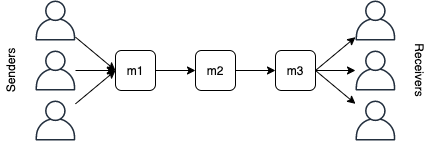
\includegraphics[width=\textwidth]{figures/topologies/cascade.png}
        \caption{Cascade}
        \label{fig:cascade}
    \end{subfigure}
    \hfill
    \begin{subfigure}[b]{0.45\textwidth}
        \centering
        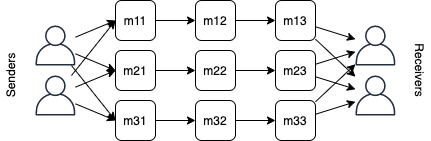
\includegraphics[width=\textwidth]{figures/topologies/multi-cascade.png}
        \caption{Multi-Cascade}
        \label{fig:multi-cascade}
    \end{subfigure}
    \hfill
    \begin{subfigure}[b]{0.45\textwidth}
        \centering
        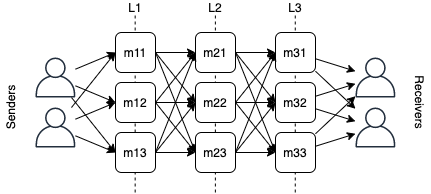
\includegraphics[width=\textwidth]{figures/topologies/stratified.png}
        \caption{Stratified}
        \label{fig:stratified}
    \end{subfigure}
    \hfill
    \begin{subfigure}[b]{0.45\textwidth}
        \centering
        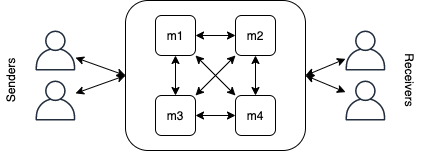
\includegraphics[width=\textwidth]{figures/topologies/mesh.png}
        \caption{Mesh}
        \label{fig:mesh}
    \end{subfigure}
       \caption{Mixnets Topologies}
       \label{fig:mixnets-topologies}
\end{figure}

\section{Mixing Techniques}

\subsection{Time-Based}
The time-based mixing technique aims to collect incoming messages and permute
and forward them every t seconds\cite{diaz2003generalising}, where t is a
system-defined variable. Figure \ref{fig:timed-mix} illustrates how time-based
Mixes work. The advantage of this mixing technique is the control of the message
transfer delay. Nonetheless, on the downside, we do not know and govern how many
messages we mix. This is because a different number of messages may be received
in separate rounds. As a result, the number of messages shuffled each time is
not the same; therefore, the anonymity set can sometimes be either larger or
smaller. A small set of messages infers reduced anonymity. To keep anonymity
above a baseline, we must incorporate complementary cover traffic, which comes
with an extra computational expense.

\subsection{Threshold-Based}
Similar to time-based mixes, a threshold Mix buffers messages into a queue until
a predefined threshold is reached. Then, we shuffle and forward messages to the
next hop\cite{diaz2003generalising}. We observe a threshold Mix in Figure
\ref{fig:threshold-mix}. In contrast with timed Mixes, threshold Mixes allow us
to control the anonymity set of messages being processed. Nonetheless, this
technique has some disadvantages as well. Primarily, the problem arises when the
network does not have much traffic, and the receiving buffer does not reach its
limit shortly. As a result, message delivery will be delayed significantly,
which is not ideal for the user's experience. The solution to this pitfall is to
integrate cover traffic in order to fill a Mix with messages more frequently. As
mentioned earlier, this comes with a computational overhead. 


\subsection{Pool-Mix}
This hybrid mixing technique\cite{diaz2003generalising} derives features from
timed and threshold mixing approaches. We release a fraction of the messages
every t seconds if a threshold is reached. The bright side of this realisation
is that a message leaving the Mix can be either a new message which just entered
the pool or an old one which was not picked during the last emission. There is
no way of knowing which one was picked. Consequently, anonymity is improved. At
the same time, one could assume this feature is a bug. In other words, a message
can stack in the pool for quite some time before arriving at its destination. We
observe that this fact yields unexpected delays. Besides that, a pool Mix
requires many messages to work optimally. Therefore, this solution might need to
include cover traffic to increase the network's capacity. Figure
\ref{fig:pool-mix} illustrates a Pool Mix.

\subsection{Continous}
This mixing technique depends on a delay given by the message
sender\cite{kesdogan1998stop}. The main advantage of this approach is that
messages are not shuffled together, and therefore, there is no statistical
inference. As described in the literature, it has a memory-less
property\cite{piotrowska2017loopix}. Each message is treated individually, and
the dispatch timestamp is not affected by the arrival of any other message.
Figure \ref{fig:continues-mix} illustrates a Continous Mix.

\begin{figure}[h!]
    \centering
    \begin{subfigure}[b]{0.45\textwidth}
        \centering
        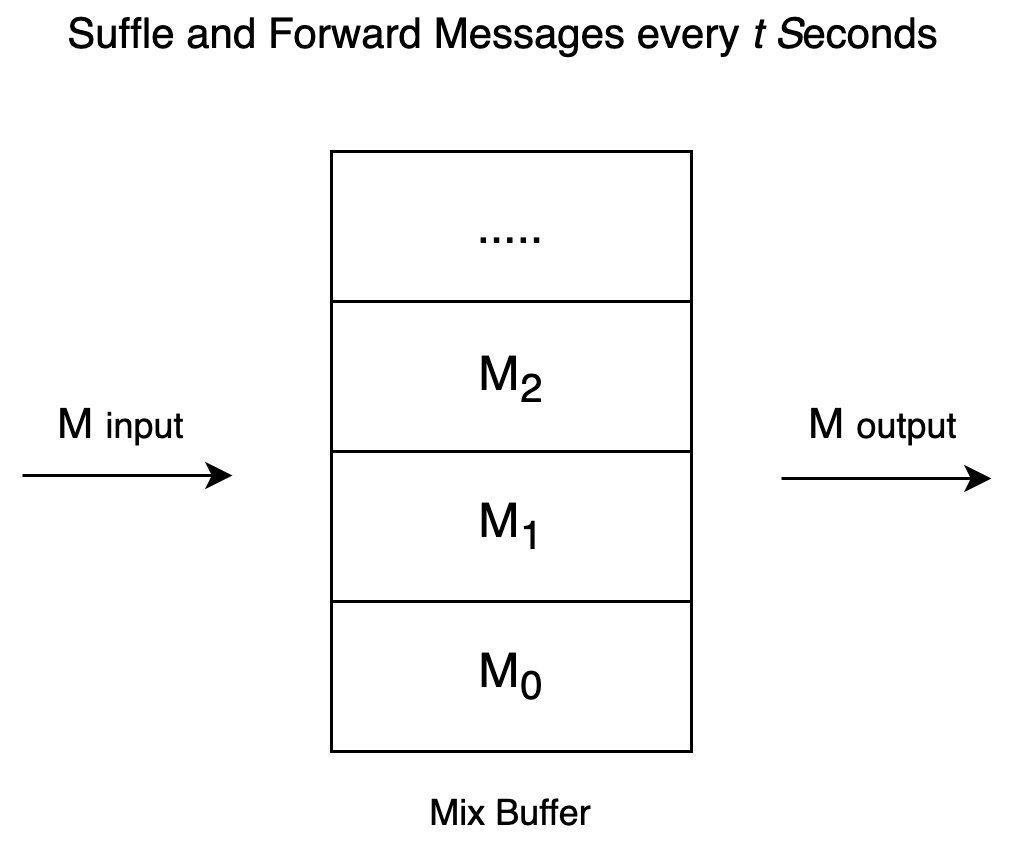
\includegraphics[width=\textwidth]{figures/mixing_techniques/timed.png}
        \caption{Timed Mix}
        \label{fig:timed-mix}
    \end{subfigure}
    \hfill
    \begin{subfigure}[b]{0.45\textwidth}
        \centering
        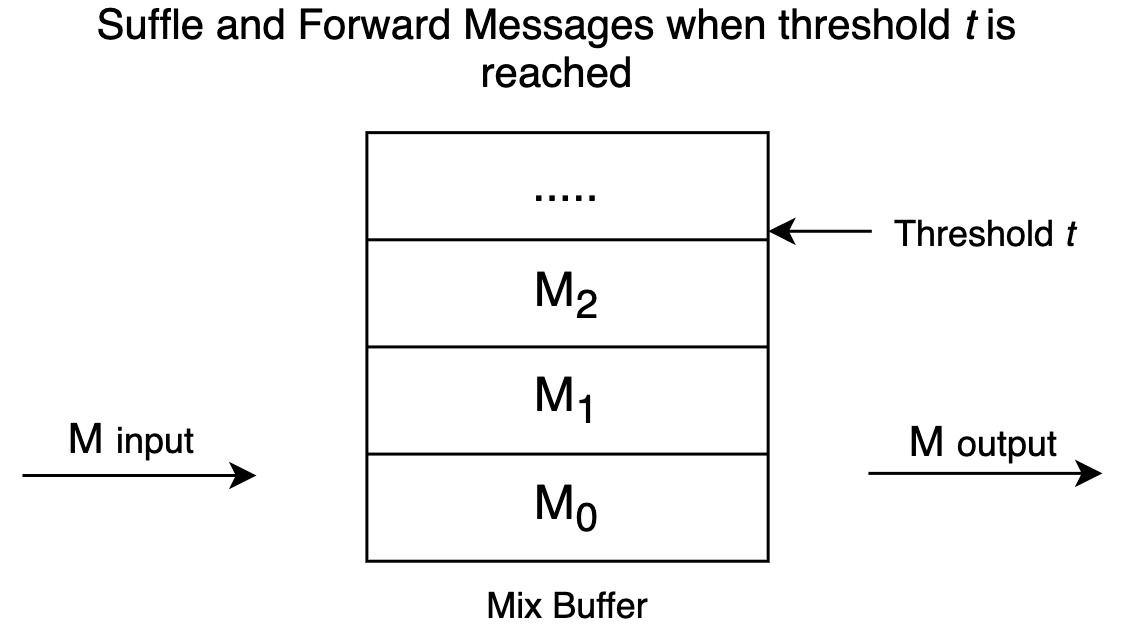
\includegraphics[width=\textwidth]{figures/mixing_techniques/threshold.png}
        \caption{Threshold Mix}
        \label{fig:threshold-mix}
    \end{subfigure}
    \hfill
    \begin{subfigure}[b]{0.45\textwidth}
        \centering
        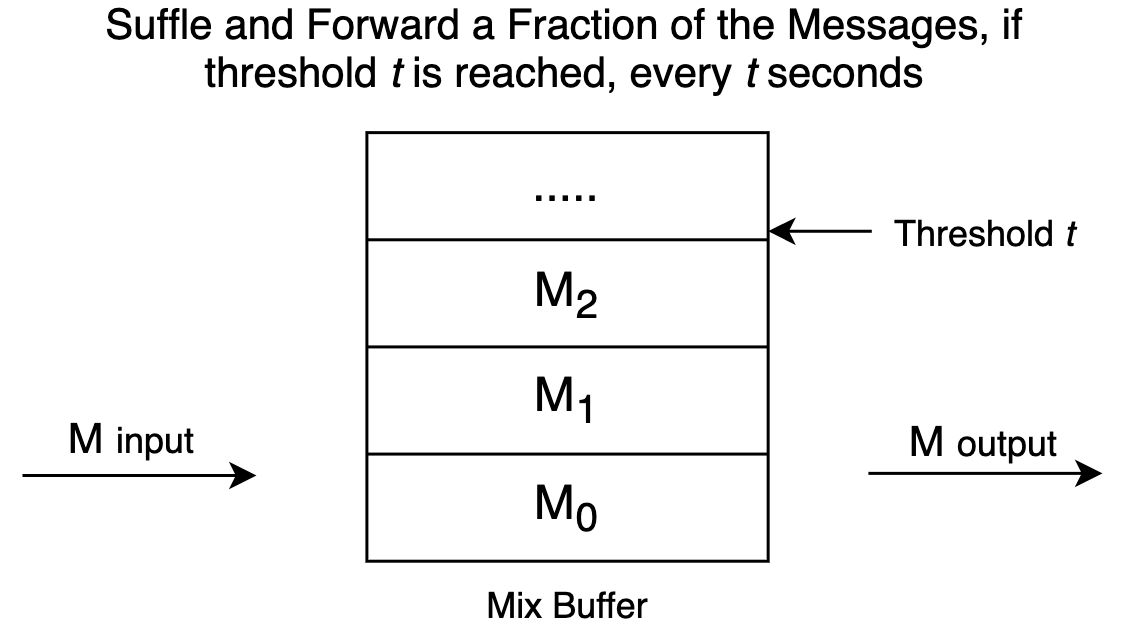
\includegraphics[width=\textwidth]{figures/mixing_techniques/pool.png}
        \caption{Pool Mix}
        \label{fig:pool-mix}
    \end{subfigure}
    \hfill
    \begin{subfigure}[b]{0.45\textwidth}
        \centering
        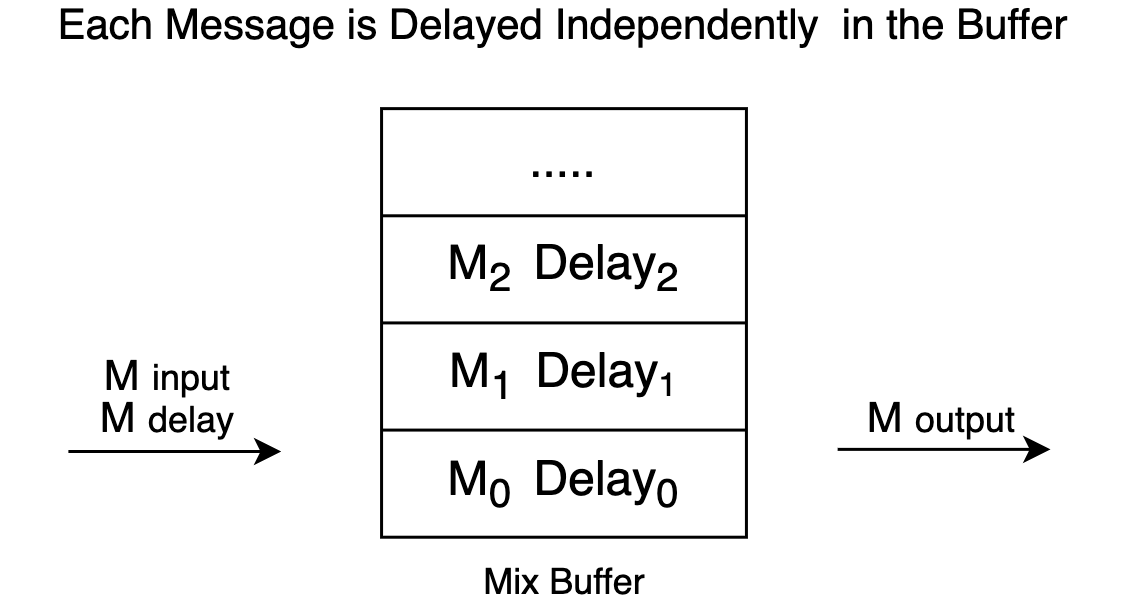
\includegraphics[width=\textwidth]{figures/mixing_techniques/continues.png}
        \caption{Continous Mix}
        \label{fig:continues-mix}
    \end{subfigure}
       \caption{Mixnets Mixing Techniques}
       \label{fig:mixnets-mixing-techniques}
 \end{figure}

\section{Measuring Anonymity}

Entropy is the natural order of the universe, meaning natural chaos. One way to
measure anonymity in Mixnets is entropy. In other words, we try to measure the
chaos among message transmissions. Even though researchers in the past defined
anonymity in various ways\cite{pfitzmann2001anonymity,
reiter1998crowds,diaz2006anonymity}, Diaz et al.\cite{diaz2002towards} and
Serjantov et al.\cite{serjantov2002towards} suggested that Shanon's
entropy\cite{entropy} is a sounder notion. Equation \ref{eq:entropy} describes
that formula. High entropy values imply better anonymity than lower values.
There is no way of identifying acceptable entropy levels since this depends on
the network size and adversary capabilities. In the following formula, we denote
as $p(x)$ the probability that an attacker can assign to a user being the
message sender. For instance, if we have an anonymity set of 1000
indistinguishable messages within a Mix buffer, we have 9.96 bits of entropy.
($Entropy = -\sum_{i = 1}^{1000}p(\frac{1}{1000}) \log_2p(\frac{1}{1000}) = 9.96
bits$). 

\begin{equation}
    \label{eq:entropy}
    H(X) = -\sum_{x \in X} p(x) \log_2p(x)     
\end{equation}

\chapter{A Deep Dive Into The Simulators}

This chapter describes MiXiM and Simulator, criticising both projects
qualitatively and quantitatively. Next, we provide information about the
simulators' realisation, development decisions, execution workflow and supported
features. We also conduct a baseline experiment, measuring their needs for
computational resources. Finally, we aggregate this information on a competitive
grid to decide which software is potentially the best to adopt for future
research and development. 

\section{Simulator}
Piotrowska's work\cite{simulator} focuses on creating a simulator for evaluating
the anonymity, latency, bandwidth overhead and scalability of Mix Networks over
different design configurations. Her study mainly used the Simulator to compare
existing projects - Elixxir\cite{xx-netowrk}, HOPR\cite{hopr} and Nym\cite{nym-tech}
- deployed on Mix Network infrastructure with different layouts.

The developed software, is based on Simpy\cite{simpy}, and realises many
features that capture real-world use cases of Mix Networks, but it is not
limited to it. Even though the simulator can handle peer-to-peer (P2P) network
simulations, we are not interested in such network formations within the context
of this project. Next, we will look deeper into the Simulator's intrinsics,
reporting on its core functionality, available features and input parameters.
Additionally, we will run the simulator against a baseline configuration file
using profiling tools\cite{cProfile,memprofiler} and capture useful information
about the simulation execution. This type of information will subsequently
enable us to comment on simulation bottlenecks.

After analysing Piotrowska's simulator, we understood the code intrinsics and
captured its approach when simulating a network. The project is well-designed,
with the main simulation entities abstracted into classes. In particular, there
are abstractions for the following entities: (a) Network, (b) Mix Node, (c) Client,
(d) Message and (e) Packet. Even though it appears to exist a provision for
splitting messages into packages, it seems that this part of the code is
incomplete, and consequently, all messages are of one packet size.

Furthermore, this simulator allows users to run experiments given many options.
Specifically, there is support for many topologies, such as (a) Cascade, (b)
Multi-Cascade, (c) Stratified and (d) P2P. In addition, there is an option for two
mixing techniques (a) batch and reorder - threshold - and (b) poisson mixing
- Continous. The current implementation has default-enabled cover traffic
generation for both clients and Mixes. Finally, the Simulator outputs the
anonymity metrics of entropy and unlinkability.

\subsection{Execution Workflow}

The workflow of executing a standard simulation scenario is as follows:

\begin{enumerate}
    \item Read user-generated configuration file.
    \item Initialize global/environment variables.
    \item Initialize loggers.
    \item Create and initialize a Network object comprising a set of clients and Mix Nodes.
    \item Randomly select two message senders and one recipient from the clients' set.
    \item All clients begin generating cover traffic, while the initially
    elected senders will also generate real traffic. The message routing is
    selected randomly on every packet hop. The current step is simulated for
    three phases, burnin, execution, and cool down. During the burnin step,
    clients and Mixes generate only cover traffic, and no logging is performed.
    On the other hand, logging is enabled during the execution stage. During
    that phase, clients and Mixes send both real and cover traffic. We log
    entropy for every real message on every hop. Lastly, we stop sending real
    messages during the cool-down phase while we continue sending dummy
    messages.
    \item Ultimately, the Simulator presents results to the user after
    inspecting the execution logs.
\end{enumerate}

\subsection{Input Parameters and Configuration File}

To begin with, the Simulator takes as input some command-line arguments,
defining the simulation mode and necessary configuration and log directories.
There follows a list of the accepted command-line arguments and their
descriptions:

\begin{itemize}
    \item[] \texttt{-mode} \textbf{(required)} \textit{(string)}: This describes
    the mode in which we run the simulator. The accepted modes are \emph{test},
    \emph{test\_diff}, \emph{transcript}, \emph{synthetic traces}, and
    \emph{anon}; however, only the \emph{test} mode is entirely realised. We have no
    clue about the functionality or purpose of the other modes.
    \item[] \texttt{-exp\_dir} \textbf{(required)} \textit{(string)}: This argument
    declares the directory's path, where the Simulator will dump any experiment
    logging files.
    \item[] \texttt{-config\_file} \textbf{(required)} \textit{(string)}: This is
    the path to the configuration file, describing the simulation settings.
 \end{itemize}

The following command-line arguments are declared but never actually used in the
Simulator. We assume that a future continuation of this project will frame their
purpose. These arguments are \texttt{-test}, \texttt{-datadir}, \texttt{-hour},
\texttt{-12hour}, \texttt{-minute}, \texttt{-day}.

Moving to the configuration file, we can observe nine sections describing
different simulation aspects. We present a sample configuration file in Appendix \ref{appendix:a1}

\textbf{Section 1} - \emph{Experiment Id}: In this section, we provide a simple
label to help keep different simulations in order.
    
\textbf{Section 2} - \emph{Logging}: This section allows us to enable or disable
logging. The attribute \texttt{dir} extends the logging directory path specified
in the command-line arguments. The attributes \texttt{client\_log} and
\texttt{mix\_log} shown in the configuration sample are never used throughout
the simulation.

\textbf{Section 3} - \emph{Simulation Phases}:  This section is related to
simulation phases - burnin, execution and cool down. Mainly we can define the
duration of each stage.

\textbf{Section 4} - \emph{Network Topologies}:  This part of the file describes
the supported network topologies of the simulator - Cascade, Stratified,
Multi-Cascade and P2P - and their properties, such as the number of layers and
layer size for stratified topologies or length and wideness for
Cascade/Multi-Cascade topologies.

\textbf{Section 5} - \emph{Packets}: This section defines the packet size
(feature not realised).

\textbf{Section 6} - \emph{Messages}: This section defines the message size
(feature not realised, all messages are of length one packet).

\textbf{Section 7} - \emph{Mixing Configurations}: This section describes Mixes'
settings like the average delay before sending a packet (Continous mixing) and
the batching of messages according to specific batch size (threshold mixing). 
    
\textbf{Section 8} - \emph{Clients Information}: This section specifies
information about clients such as the number of participating clients, how
often the client adds a real message to the send buffer, the send rate, and if
the client is generating cover traffic, and if so, at what rate. It is important
to note that the attributes \texttt{rate\_ack}, \texttt{ACK},
\texttt{retransmit}, \texttt{dummies\_acks}, and \texttt{max\_retransmissions}
are never used. 

\textbf{Section 9} - \emph{miscellaneous}: This section
denotes the length of a message-id and the number of total real messages we
want to send during the simulation.


\subsection{Baseline Simulation and Profiling Measurements}

In our endeavour to assess Simulator, we run a series of experiments to identify
its performance and quality of results. In particular, the baseline simulation
examines the Simulator's behaviour in terms of space, memory, time complexity,
and the network's entropy. We run the same experiment for the three established
topologies - Cascade(10 Mixes), Multi-Cascade (3x10 Mixes) and Stratified (3x10
Mixes) - while increasing the simulation duration from 100 to 10000 time ticks.
We also configured the mixing technique to Poisson (i.e. Continous), the number
of clients to 100, and set the number of real messages under transfer to 1000. 

Our anticipation regarding memory usage assumes all experiments will deliver the
same results for all topologies except Cascade. We establish our assumption on
the fact that a single Cascade topology has fewer Mixes than the other
topologies described earlier. However, according to Figure
\ref{fig:baseline-mem}, our hypothesis fails since the Simulator uses the same
amount of memory - roughly 247 megabytes - in all experiments. In a later
chapter, we will point out that memory usage solely depends on the number of
users we simulate.

In regards to space complexity, we expect to have differences among topologies.
Specifically, a Cascade Mixnet needs to route traffic through a chain of nodes.
The network's capacity aligns with a single mix's capacity. Therefore, every
time we dump each Mix's logs, we observe log lines to repeat because messages
stall there for a long time. A Multi-Cascade Mixnet performs better since there
are parallel chains of Mixes. The Stratified topology should be the best since
messages continually move from one Mix to another and do not repeat in the log
files. Indeed, our hypothesis is accurate, and we can notice the results in
Figure \ref{fig:baseline-space}

Execution time should follow the same pattern as space complexity, given the
same reason concerning the nature of each topology, as noted previously. We
observe in Figure \ref{fig:baseline-time} that this is mostly true, except for
the Simulation duration of 1000 time ticks. This negligible time offset, on
Figure \ref{fig:baseline-time}, could be caused by other processes running on
our workstation at that moment.

Further, we need to check if Piotrowska's simulator reasonably captures the
notion of entropy for each topology. According to our measurements in Figure
\ref{fig:baseline-entropy}, Simulator reports higher entropy for Cascade
topology. There follows Multi Cascade and Stratified. These results are
acceptable since aggregating more messages on each hop increases Mix's anonymity
set, so entropy is higher.

\begin{figure}[h!]
    \centering
    \begin{subfigure}[b]{0.45\textwidth}
        \centering
        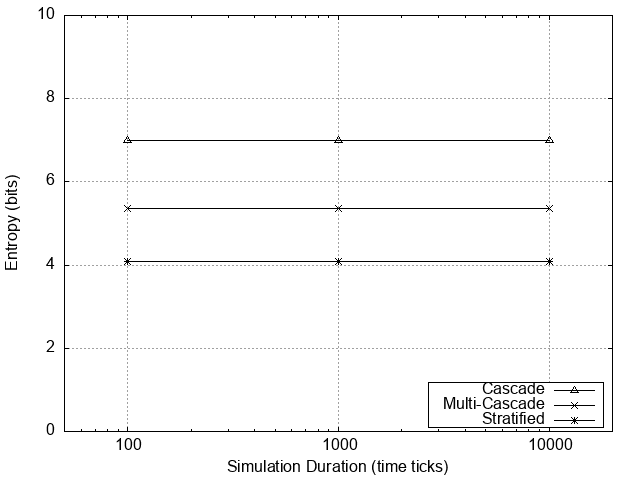
\includegraphics[width=\textwidth]{figures/baseline_simulation/simulator/baseline_simulator_entropy.png}
        \caption{Entropy}
        \label{fig:baseline-entropy}
    \end{subfigure}
    \hfill
    \begin{subfigure}[b]{0.45\textwidth}
        \centering
        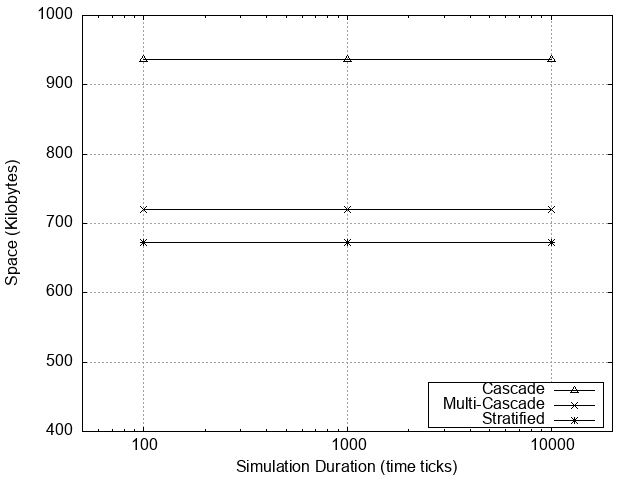
\includegraphics[width=\textwidth]{figures/baseline_simulation/simulator/baseline_simulator_space.png}
        \caption{Space}
        \label{fig:baseline-space}
    \end{subfigure}
    \hfill
    \begin{subfigure}[b]{0.45\textwidth}
        \centering
        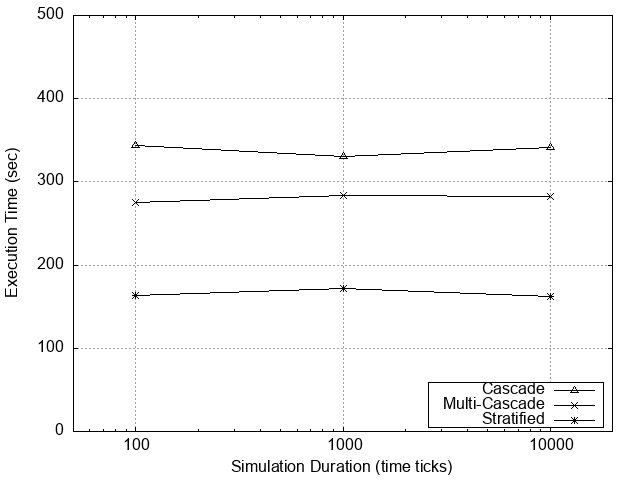
\includegraphics[width=\textwidth]{figures/baseline_simulation/simulator/baseline_simulator_time.png}
        \caption{Execution Time}
        \label{fig:baseline-time}
    \end{subfigure}
    \hfill
    \begin{subfigure}[b]{0.45\textwidth}
        \centering
        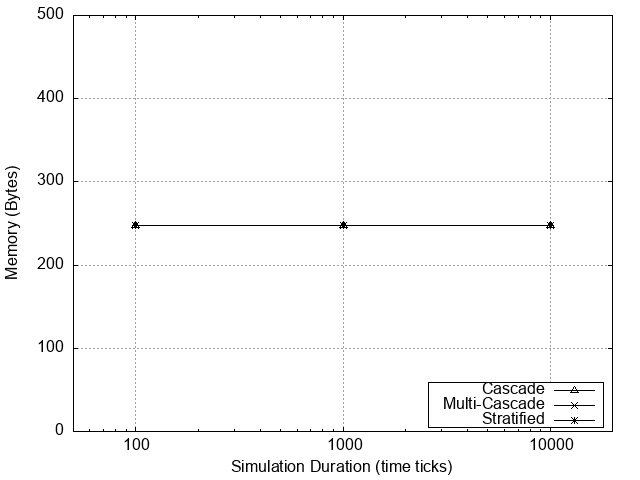
\includegraphics[width=\textwidth]{figures/baseline_simulation/simulator/baseline_simulator_mem.png}
        \caption{Memory}
        \label{fig:baseline-mem}
    \end{subfigure}
       \caption{Simulator Baseline Experiments}
       \label{fig:baseline-simulation}
 \end{figure}
 

Finally, we run Piotrowska's project using a \emph{cProfiler}\cite{cProfile} to
get visual information and statistics about its execution tree (sequence of
functions called). We get a detailed representation of the execution tree in
Appendix \ref{appendix:b1}. We also analyze the project using \emph{SonarQube}\cite{sonarqube} to
get information about the quality of the code. In the first place,
\emph{cProfiler} reveals that 59.75\% of the CPU usage was for processing
packets, while the heaviest task running under the \emph{packet processing}
branch was \emph{entropy\_update()}. \emph{entropy\_update()} took 38.76\% of
the total CPU usage, indicating a possible bottleneck to the whole execution.
Regarding \emph{SonarQube} results, we found out that 2.7\% of the code is
duplicated, and there are 57 \emph{code smells}, 2 \emph{bugs} and 5
\emph{security issues} of no great importance.

\section{MiXiM}

Guirat et al.\cite{guirat2022mixnet} carried out a similar attempt to develop an
event-driven Mix Network simulator using Simpy\cite{simpy}. In particular,
their study\cite{guirat2022mixnet} presents MiXiM, a simulation framework that
helps academics and industry professionals assess various Mix Networks design
options. Next, we will delve into the simulator implementation, reporting on its
functionality, available features and input parameters. Besides that, we aim to
run the simulator against a baseline scenario, reporting on its outputs and
execution statistics. This information will help us decide if MiXiM is a
well-built and feature-proof tool that brings out the most.

After we analysed  MiXiM, we understood the code intrinsics and captured its
approach when simulating a network. Likewise, Piotrowska's work is well-designed
and abstracted into similar entities: (a) Simulation, (b) Network, (c) Mix Node -
Poisson Mix, Pool, Timed Mix, Threshold Mix - (d) Client, (e) Relay -
abstraction of an attacker - and (f) Message.


Moreover, the simulator allows users to run experiments given various
configurations. In more detail, there is support for many topologies, such as
(a) Cascade, (b) Multi-Cascade, and (c) Ctratified. Additionally, there is an
option for three mixing techniques (a) Timed mixing and (b) Poisson mixing, (c)
Threshold Mixing and (d) stop-and-go mixing\cite{kesdogan1998stop} (i.e.
Continous). Besides that, the users can enable dummy traffic generation, giving
a specific generation rate. Another outstanding feature is the introduction of
corrupted mix nodes during the simulation. Finally, the Simulator outputs the
anonymity metric of entropy.

\subsection{Execution Workflow}

The workflow of executing a standard simulation scenario is as follows:

\begin{enumerate}
    \item Read user-generated configuration file.
    \item Create and initialize a simulation object passing all the input
    parameters found in step 1.
    \item Call the run function of the simulation object.
    \item Create and initialize a Network object comprising a set of Clients and
    Mix Nodes, including possible corrupted nodes. Connect nodes with their
    neighbours.
    \item All clients begin generating traffic according to the given $\lambda$
    generation variable. In the meantime, dummy traffic is generated as well.
    \item The simulation is executed in a single phase lasting for several time
    ticks declared in the configuration file. During each message transmission
    from one node to another, entropy is updated.
    \item After inspecting the execution logs, MiXiM presents the entropy to the user.
\end{enumerate}

\subsection{Input Parameters and Configuration File}

MiXiM, compared to Simulator, does not take any command-line arguments. We only
observe a single configuration file with six different sections. We present a
sample configuration file in Appendix \ref{appendix:a2}. Following, we provide a thorough
description of the aforementioned file.

\textbf{Section 1} - \emph{DEFAULT}: Under the DEFAULT section, we recognise
the number of clients sending and receiving messages in a network and a
parameter called lambda\_c representing the rate of generating messages per time
tick. 

\textbf{Section 2} - \emph{TOPOLOGY}: In this section, we describe settings for
all three supported topologies - Stratified, Cascade and Free Route. The
parameter fully\_connected enables us to have a complete or a semi-connected
Stratified topology. Also, we define the routing strategy by choosing between
the \texttt{source} - users choose the route - or \texttt{hop\_by\_hop} - random
selection. Other parameters include \texttt{E2E}, the minimum end-to-end
transmission delay, and \texttt{n\_layers}, \texttt{l\_mixes\_per\_layer} and
\texttt{n\_cascades}, which describe the number of layers and their
corresponding number of mixes.

\textbf{Section 3} - \emph{MIXING}: This section is related to the available
mixing techniques. We have the \texttt{mix\_type}, which can be Poisson, Time,
or Pool and mu, which is the delay on each mix node. For each of the
aforementioned mixing techniques, the variables timeout, threshold, and
\texttt{flush\_percent}, match each case accordingly.

\textbf{Section 4} - \emph{DUMMIES}: This section regards dummy data generation.
The user sets the variables \texttt{client\_dummies} to enable or disable dummy
messages, \texttt{rate\_client\_dummies} to control the dummy data generation,
\texttt{link\_based\_dummies} to send dummies dropped on the next hop,
\texttt{multiple\_hop\_dummies} to send dummies that last for many hops, and
\texttt{rate\_mix\_dummies} to generate dummy messages on the Mix.

\textbf{Section 5} - \emph{NODE\_SELECTION}: All attributes in this
section are not required during the simulation and might be the fragments of
older software versions. 

\textbf{Section 6} - \emph{THREAT\_MODEL}: In this section we define the number
of corrupted nodes and we give direction weather we want them to be uniformly
distributed across the network layers.


\subsection{Baseline Simulation and Profiling Measurements}

Section 3.1.3 described our attempt to evaluate the Simulator according to a
baseline scenario. We make the same assumptions for MiXiM, running the same
experiments. Unfortunately, our expectations do not match the results since we
could not reproduce every simulation.

Mainly, we managed to simulate Stratified topologies for 100 and 1000 time
ticks. Attempting to run experiments for Cascade and Multi-Cascade network
arrangements failed due to run-time errors. Simulating a Stratified topology for
10000 time ticks resulted in a crash too. We were hesitant about the failure
causes, so we decided to probe the software code-base to uncover potential
issues.

Indeed, skimming the source code, we managed to spot four bugs we present in the following list: 

\begin{enumerate}
    \item The parsing section of the code accepts as valid topologies "cascade",
    "multi-cascade", and "stratified". Nevertheless, this is not the case for
    some files - Network.py, Simulation.py and Client.py - where the code
    expects a topology called "XDR". This contradiction causes MiXiM to crash,
    given the topologies "cascade" and "multi-cascade". 
    \item The variable n\_cascade, which describes the number of parallel
    Cascades in Network.py, is hard coded. Hence, the simulation is not assuming
    the user's configuration.
    \item In file Simulation.py, a variable is declared as \emph{otherClient}, while
    the software developer used the name \emph{other\_client} when initialising the
    variable. Consequently, the initialisation is meaningless, and \emph{otherClient}
    has no value.
    \item The initial parsing of boolean parameters from the configuration file
    is incorrect since the code used is a Python2 command which, when using
    Python3 - other project libraries require it - always returns True.
    Therefore, all boolean parameters in the configuration file are True, no
    matter their actual value.
\end{enumerate}

The purpose of this project is not to fix someone else's work but to assess
it. Consequently, we did not proceed with further code reviews or repairs.

In regards to the successful experiments, we can observe the results in Figure
\ref{fig:baseline-mixim-simulation}. Surprisingly, the execution time and space
used to dump log files increase linearly for different simulation time-frames.
According to our previous code analysis, this is justifiable since clients in
MiXiM generate messages based on predefined $\lambda$ rate. The longer the
simulation, the more messages are generated. Hence, more processing time and
storage space are required.

On the other hand, Simulator uses only the number of specified target messages
regardless of the duration. Furthermore, it is notable that in terms of memory
usage, MiXiM is sufficient, requiring only 21.4 MB of RAM for all our
successful trials. We cannot deduce further valuable insights from these
graphs because, as we mentioned earlier, we failed to perform all baseline
experiments.

Ultimately, we run the project using a cProfiler to get visual information and
statistics about the execution tree. We get a detailed representation of the
execution tree in Appendix \ref{appendix:b2}. We also analyze the project using
\emph{SonarQube} to obtain information about the quality of the code. In the first
place, cProfiler reveals that 44.18\% of the CPU usage was for randomly
selecting the next hop of a packet. MiXiM's case is different from Piotrowska's
Simulator, in which updating entropy was the most resource-hungry task. In fact,
this happens because MiXiM calculates entropy at the end of the simulation,
using the message logs. Regarding \emph{SonarQube} results, we find out that 0\%
of the code is \emph{duplicated}; however, there are 81 \emph{code smells} and
10 \emph{security issues} that are not of great importance.


\begin{figure}[h!]
    \centering
    \begin{subfigure}[b]{0.45\textwidth}
        \centering
        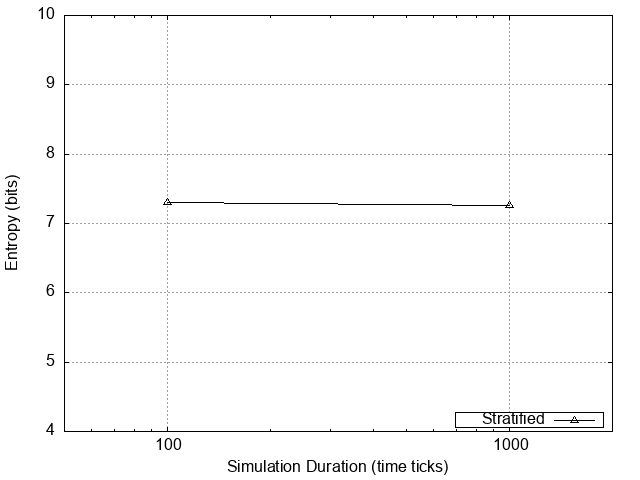
\includegraphics[width=\textwidth]{figures/baseline_simulation/mixim/baseline_mixim_entropy.png}
        \caption{Entropy}
        \label{fig:baseline-mixim-entropy}
    \end{subfigure}
    \hfill
    \begin{subfigure}[b]{0.45\textwidth}
        \centering
        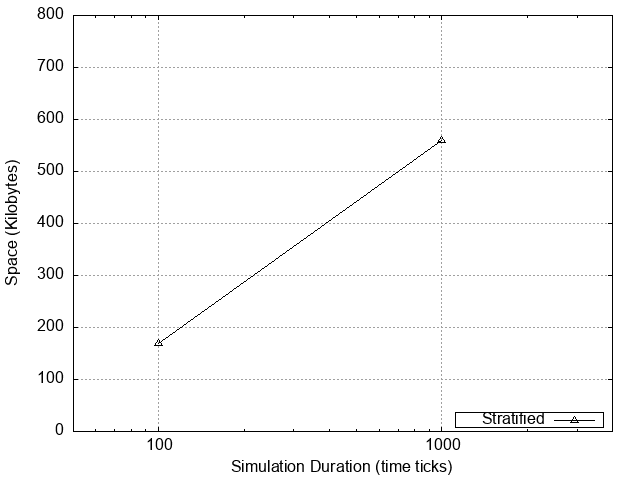
\includegraphics[width=\textwidth]{figures/baseline_simulation/mixim/baseline_mixim_space.png}
        \caption{Space}
        \label{fig:baseline-mixim-space}
    \end{subfigure}
    \hfill
    \begin{subfigure}[b]{0.45\textwidth}
        \centering
        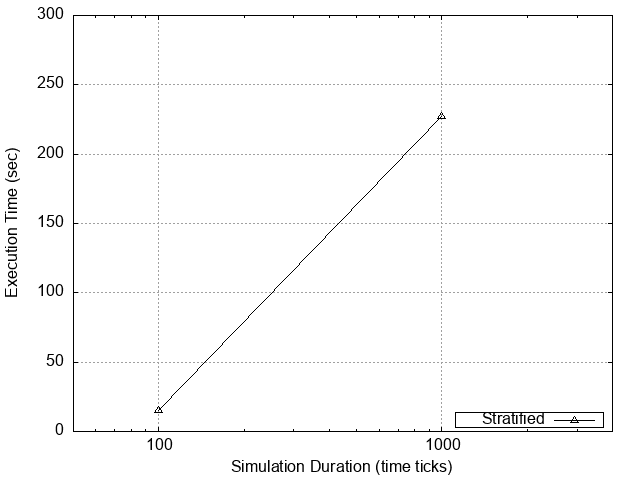
\includegraphics[width=\textwidth]{figures/baseline_simulation/mixim/baseline_mixim_time.png}
        \caption{Execution Time}
        \label{fig:baseline-mixim-time}
    \end{subfigure}
    \hfill
    \begin{subfigure}[b]{0.45\textwidth}
        \centering
        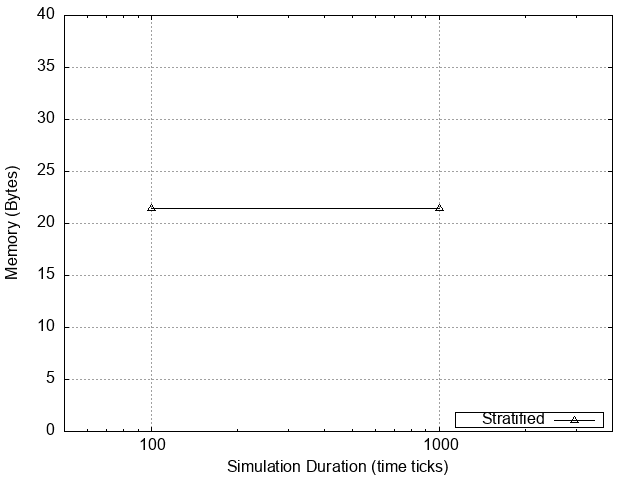
\includegraphics[width=\textwidth]{figures/baseline_simulation/mixim/baseline_mixim_mem.png}
        \caption{Memory}
        \label{fig:baseline-mixim-mem}
    \end{subfigure}
       \caption{MiXiM Baseline Experiments}
       \label{fig:baseline-mixim-simulation}
 \end{figure}


\section{Compasisson Framework}

To bring conclusiveness to our simulators analysis, we present in this section a
comparison framework. Our ultimate goal is to find out which simulator is better
to adopt for further development in the future. A comprehensive comparison
framework needs to evaluate multiple factors. Therefore, we assumed the following
KPIs (key performance indicators) (a) Topologies, (b) Mixing Techniques, (c)
Routing Methods for Stratified topology, (d) Cover Traffic, (e) Corrupt Relays,
and (f) SonarQube Code analysis insights.

\begin{table}[h!]
    \begin{center}
        \begin{tabular}{||c|l|c|c||}
            \hline
                                                                &                               & Simulator   & MiXiM         \\ \hline
            \multirow{5}{*}{Topologies}                         & Cascade                       & \ding{51}   & \ding{51}         \\ \cline{2-4} 
                                                                & Multi-Cascade                 & \ding{51}        & \ding{51}          \\ \cline{2-4} 
                                                                & Stratified - Fully Connected  & \ding{51}        & \ding{51}          \\ \cline{2-4} 
                                                                & Stratified - Semi Connected   &               & \ding{51}          \\ \cline{2-4} 
                                                                & P2P                           & \ding{51}       &                  \\ \hline \hline
            \multirow{4}{*}{Mixing Techniques}                  & Timed                         &                & \ding{51}          \\ \cline{2-4} 
                                                                & Threshold                     & \ding{51}       & \ding{51}          \\ \cline{2-4} 
                                                                & Pool                          &                & \ding{51}          \\ \cline{2-4} 
                                                                & Continous                     & \ding{51}      & \ding{51}          \\ \hline \hline
            Routing                                             & Random Choice                 & \ding{51}      & \ding{51}         \\ \hline \hline
            \multirow{3}{*}{Cover Traffic}                      & On Client                     & \ding{51}       & \ding{51}         \\ \cline{2-4} 
                                                                & On Mix                        & \ding{51}       & \ding{51}         \\ \cline{2-4} 
                                                                & Multi-hop Dummies             &                & \ding{51}         \\ \hline \hline
            Relays                                              & Corrupt Mixes                 &                & \ding{51}          \\ \hline \hline
            \multirow{7}{*}{Code Analysis}                      & Code Readability              & 4/5            & 2/5              \\ \cline{2-4}
                                                                & Object Abstraction            & 5/5             & 5/5               \\ \cline{2-4}
                                                                & Code Smells                   & 57            & 81                \\ \cline{2-4}
                                                                & Bugs                          & 2             & 4                  \\ \cline{2-4}
                                                                & Security Issues               & 5              & 10                \\ \cline{2-4}
                                                                & Duplicate Code                & 2.7\%        & 0\%               \\ \cline{2-4}
                                                                & Runtime Crashes               &                  & \ding{51}            \\ \hline \hline
            \end{tabular}
    \end{center}
    
    \caption{Simulators Comparisson Table}
    \label{tab:comparisson-table}
    \end{table}

Table \ref{tab:comparisson-table} illustrates how MiXiM and Simulator are
compared in each aspect. We notice that MiXiM realises 13 features, while
Simulator has only 9. Nonetheless, it is essential to prompt that most of
MiXiM's features do not work, crashing on runtime. Also, both software achieve
high scores in object abstraction, while code readability for MiXiM seems to be
poor. Further, MiXiM has 81 \emph{code smells} compared to Simulator, which  has
only 57 \emph{code smells}. Moreover, MiXiM has double the \emph{bugs} and
\emph{security issues} compared to Simulator, which has 2 and 5, respectively.
Eventually, both projects have negligible amounts of \emph{code duplication}.

Ultimately, we decided that the best simulator, so far, is Piotrowska's
Simulator. We justify our decision mainly based on the usability aspect. Even
though MiXiM advertises a large set of features, it fails to deliver a working
code-base. We are confident that Simulator is a well-designed software and can
be improved by supporting a complete set of features, in the future. Besides,
Simulator justifies our reasoning for valid and quality entropy and network
latency results. 

\chapter{Replication Study}
This chapter is dedicated to replicating existing
literature\cite{piotrowska2021studying,ben2021mixim}, reasoning about its
outcomes. Minutely, a replication study frames the process of reproducing and
analysing the experiments of other researchers under similar conditions. The
purpose of a replication study is primarily to discover if current findings
provide a valid basis for deciding future research paths.

Within the context of this dissertation, we conduct a short replication study,
considering previous works\cite{piotrowska2021studying,ben2021mixim}. Our goal
is to realise how existing topologies, mixing techniques, cover/decoy traffic
and the appearance of corrupter Mixes affect the latency and anonymity of a
Mixnet. This analysis will help us reason about Mixnets' behaviour, further
extending recent research in Chapter 5.

Replicating previous work was challenging for many reasons. For our part, the
experimental set-up was not clearly described, and some parameters were missing.
Consequently, we had to make assumptions on a few occasions. Another essential
aspect when replicating studies is to use similar environments. Nonetheless,
none of the previous research had references to the employed hardware. For this
reason, we used our personal computer, comprising an Ubuntu machine facilitating
a 6-core Intel core i5-8600K and 16 GB of RAM. The experiments conducted
throughout chapters 4 and 5 use exclusively this equipment. At this point, it is
worth mentioning that simulating more than 4000 clients on Piotrowska's
Simulator required more than 16 GB of RAM, which was out of our practical limit.
Therefore, we managed to replicate most of the experiments partially. 

\section{Studying the Effect of Mix Network Topologies and Mixing Techniques}

Indubitably, different topologies and mixing techniques, as described in chapter
2, can impact the anonymity and latency of a Mix Network. Piotrowska saught the
same questions when writing her study on the anonymity
trilemma\cite{piotrowska2021studying}. The conducted experiments evaluated and
compared three Mixnets implementations - Nym, Elixxir Network, and HOPR. Each
one of these projects is designed using a different topology. 

Nym integrates a stratified topology based on three layers with three Mixes
each. Also, the mixing technique used is Continous, where the delay is randomly
picked from the exponential distribution. On the other hand, Elixxir is a
Chaumian cascade network based on the cMix protocol\cite{chaum2017cmix}. Elixxir
can be configured to run on a single Cascade, like cMix, or use multiple
Cascades. Compared to Nym, Elixxir uses the batch and reorder mixing technique
(for Elixxir Network, we assumed a 1000 message threshold). Lastly, HOPR uses a
P2P topology, and for this reason, we did not include it in this work.


In the first place, we are going to compare Single-Cascade and Multi-Cascade
network topologies. Intuitively, we expect that a Single-Cascade formation will
have higher anonymity levels since all traffic is routed through a chain of
Nodes. Shuffling the whole anonymity set of messages on each stop can provide
greater anonymity. Nonetheless, we assume that latency can be high because the
network's capacity is caped to the Mix's throughput. The latency can be low for
a negligible number of clients, but it will be higher if we increase the user
base.

\begin{figure}[h!]
    \centering
    \begin{subfigure}[b]{0.45\textwidth}
        \centering
        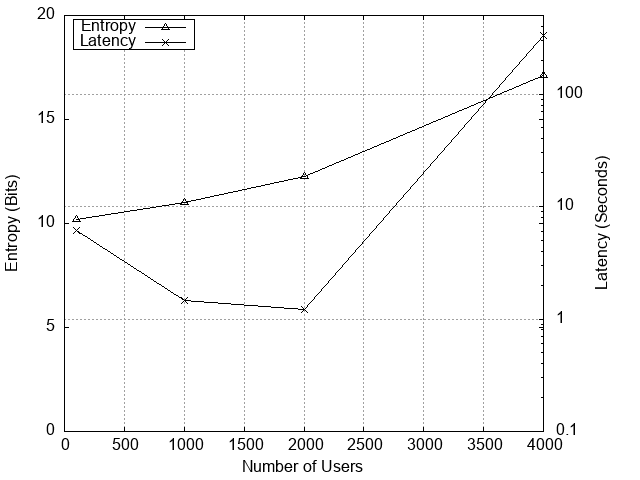
\includegraphics[width=\textwidth]{figures/simulator/1_a.png}
        \caption{Single-Cascade Elixxir Network}
        \label{fig:elixxir-cascade}
    \end{subfigure}
    \hfill
    \begin{subfigure}[b]{0.45\textwidth}
        \centering
        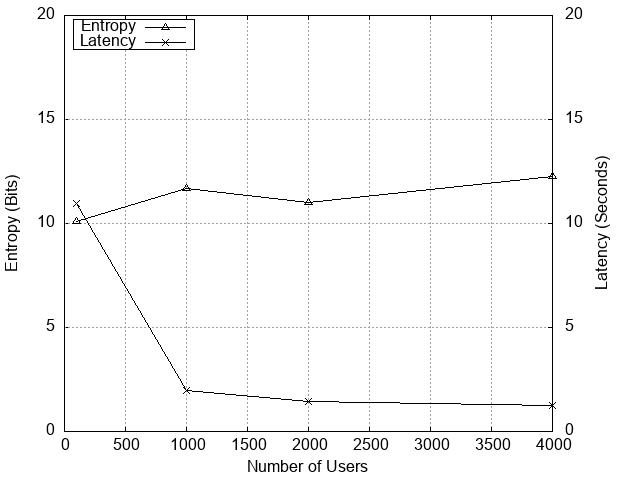
\includegraphics[width=\textwidth]{figures/simulator/1_b.png}
        \caption{Multi-Cascade Elixxir Network}
        \label{fig:elixxir-multi-cascade}
    \end{subfigure}
       \caption{MiXiM Baseline Experiments}
       \label{fig:elixxir}
 \end{figure}


 Figure \ref{fig:elixxir} portray the expected results. Assuming
 Cascades of length three and by increasing the number of users, we observe an
 increase in entropy as well. Also, we notice that the entropy's increase rate
 is much more extensive for a Single-Cascade (1x3) than for a Multi-Cascade(2x3)
 topology. Nonetheless, there is evidence of poor latency in Figure
 \ref{fig:elixxir-cascade} when the system facilitates more than 2000 users.
 Latency sharply increases from just above 1 second to almost 350 seconds. On
 the other hand, a Multi-Cascade design allows very low latency by sacrificing a
 bit of anonymity. From the above analysis, we can deduce that for Cascade and
 Multi-Cascade topologies, we have to choose between scalability and anonymity.
 We can not have both.

 In contrast to Cascade topologies, a Stratified topology should scale better.
 This is intuitive since we can add more Mixes to each layer, distributing
 traffic into distinct routes. At the same time, we deem it is possible to
 achieve lower latency since not many messages get congested into a Mix. 

 As we notice in Figure \ref{fig:nym-stratified}, Nym's Stratified
 implementation - three layers of three Mixes each - can achieve greater anonymity with
 very low latency. We presume that latency is at the level of 0.3 seconds
 because Nym realises a Continous mixing technique, while earlier, Elixxir used
 a batch and reorder technique, meaning that batch size can affect latency.
 Moreover, entropy is in an uptrend, showing that by increasing the number of
 users, anonymity increases as well. Therefore, Nym's Stratified configuration
 can handle significant traffic with increasing anonymity and low latency.

\begin{figure}[h!]
    \centering
    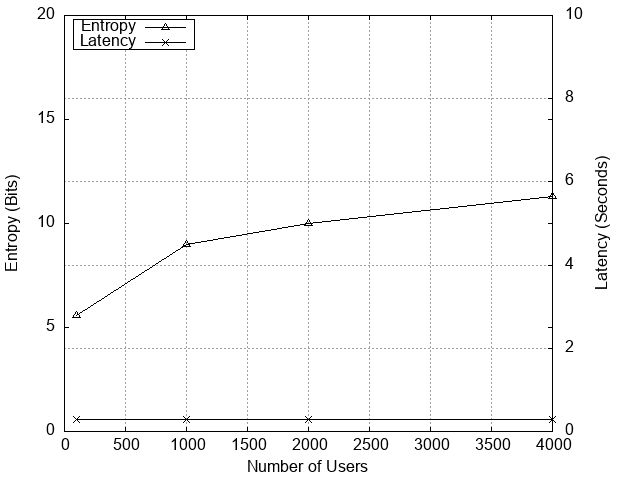
\includegraphics[height=8cm]{figures/simulator/2.png}
    \caption{Stratified Nym Network}
    \label{fig:nym-stratified}
 \end{figure}

 Using MiXiM, we get similar results. In particular, Figure
 \ref{fig:mixim-different-generation} depicts the anonymity of a Stratified
 topology of three layers comprising ten Mixes each, simulated by setting the
 $\lambda$ message generation factor to 1 and 10, respectively. We observe that
 entropy increases when traffic rises, conforming to the previous experiment's
 results.

 Also, Figure \ref{fig:mixim-different-layers} shows us the impact on entropy
 when increasing the number of layers, assuming different average delays on
 mixing - presuming Continuous mixing. We observe anonymity growing between one
 and two layers; however, there is a steady decline afterwards. We are not sure
 why this happens. Intuitively, the longer the route a message takes, the bigger
 should be the entropy. Besides, assuming various mixing delays, the entropy
 should have been higher for more extended time frames. According to the
 simulation results, this is not true, as the drawn curves seem primarily
 identical. Nonetheless, we are not confident about the quality of the results
 since, as we have studied in Chapter 3, MiXiM has many bugs and unrealised
 features.

\begin{figure}[h!]
    \centering
    \begin{subfigure}[b]{0.45\textwidth}
        \centering
        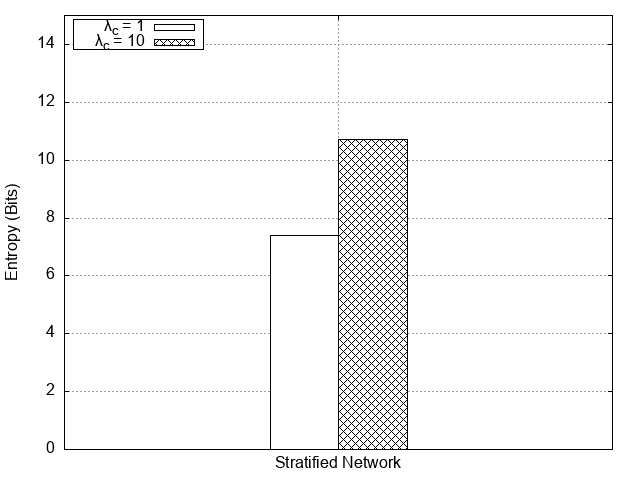
\includegraphics[width=\textwidth]{figures/mixim/2.png}
        \caption{Impact of different messages generation rates on entropy}
        \label{fig:mixim-different-generation}
    \end{subfigure}
    \hfill
    \begin{subfigure}[b]{0.45\textwidth}
        \centering
        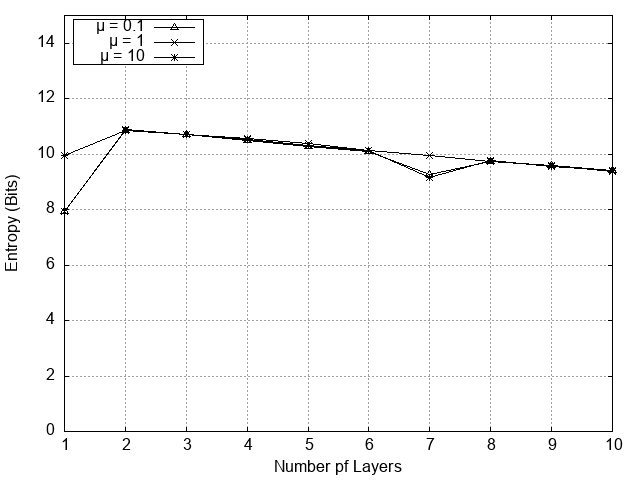
\includegraphics[width=\textwidth]{figures/mixim/3.png}
        \caption{Impact of different number of layers and average delay on Entropy}
        \label{fig:mixim-different-layers}
    \end{subfigure}
    \caption{Impact on Ananymity}
 \end{figure}

\section{Studying the Effect of Traffic}

Cover traffic is an essential tool that both MiXiM and Simulator incorporate.
Notably, using dummy messages, we increase the anonymity set during the mixing
stage. Allegedly, we anticipate greater anonymity when having more traffic.
Also, cover traffic enables us to aim for the same anonymity levels while
reducing latency. Theoretically, we achieve that by increasing traffic and
keeping the average delay low - assuming the Continuous mixing technique. 

\subsection{Cover Traffic}

Figure \ref{fig:cover-traffic-ratios} illustrates the effect of cover traffic on
anonymity, assuming different cover traffic ratios. We observe that for higher
ratios, anonymity is greater. Also, increasing the number of users contributes
to anonymity. Notably, in Figure \ref{fig:cover-traffic-decreasing-ratios} we
notice that decreasing the cover traffic ratio from 10:1,  to 2:1 [Cover:Real]
yields acceptable levels of entropy, which is further boosted by the increasing
number of users. 


\begin{figure}[h!]
    \centering
    \begin{subfigure}[b]{0.45\textwidth}
        \centering
        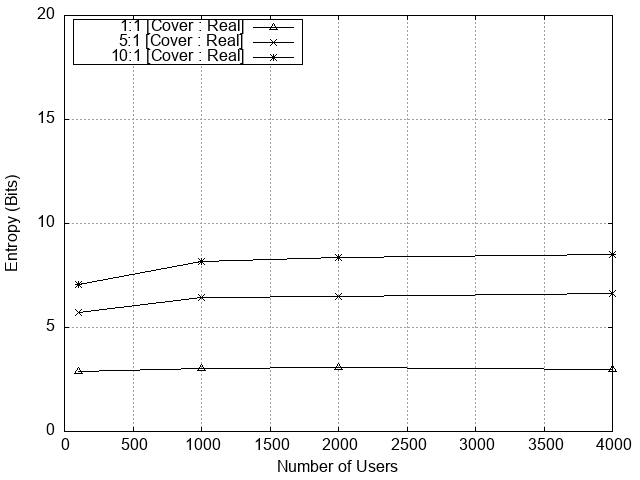
\includegraphics[width=\textwidth]{figures/simulator/3.png}
        \caption{Impact of different Cover Traffic Ratios on Entropy}
        \label{fig:cover-traffic-ratios}
    \end{subfigure}
    \hfill
    \begin{subfigure}[b]{0.45\textwidth}
        \centering
        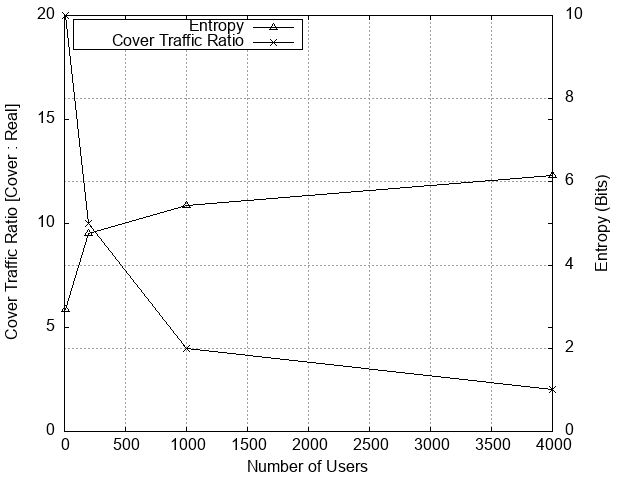
\includegraphics[width=\textwidth]{figures/simulator/4.png}
        \caption{Impact of Decreasing Cover Traffic on Entropy}
        \label{fig:cover-traffic-decreasing-ratios}
    \end{subfigure}
    \caption{Impact of Cover Traffic on Anonymity}
 \end{figure}

\subsection{Real Traffic}

Real traffic is generated according to the number of users in our network.
Therefore, more users imply higher anonymity levels. In fact, as noted by
[simulator] and [mixim], increasing the average delay of Continous mixing offers
greater anonymity. Nevertheless, what if we want to keep latency down? As we
notice in Figure \ref{fig:nym-stratified-low-latency-constant-anonymity} this
can be achieved by keeping the average delay lower. As more and more users join a
Stratified network, the anonymity increases; thus, we can employ low mixing
delays. As a result, we have a network with low latency yet constant anonymity.

\begin{figure}[h!]
    \centering
    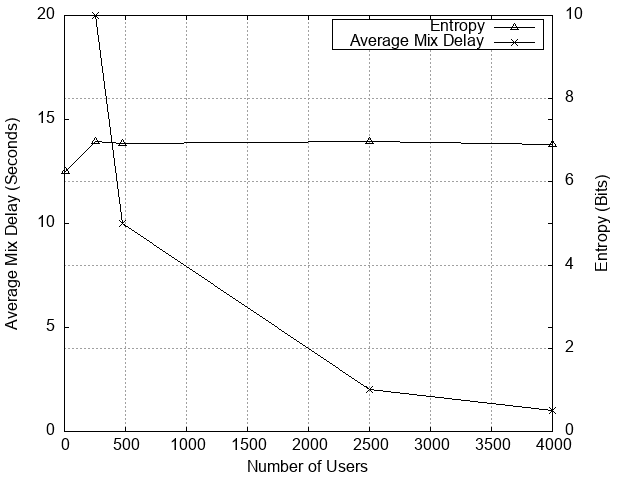
\includegraphics[height=8cm]{figures/simulator/5.png}
    \caption{Constant Entropy with reduced Latency}
    \label{fig:nym-stratified-low-latency-constant-anonymity}
 \end{figure}

\section{Studying the Effect of Corrupt Relays}

Another exciting subject investigated by Guirat et al.\cite{ben2021mixim} is the
appearance of corrupted Mixes within a Stratified network. The notion of a
corrupt node implies that the adversary knows all input and output messages on a
Mix with complete certainty. 

The results illustrated in Figure \ref{fig:corrupted-mixes} refer to a
Stratified network of three layers comprising ten mixes each. The mixing technique
used is Continous, with an average delay of 0.1 seconds. Also, we facilitate 100
clients, each generating 10 messages per second. For this experimental set-up,
we anticipate declining anonymity by increasing the percentage of corrupted
mixes. 

\begin{figure}[h!]
    \centering
    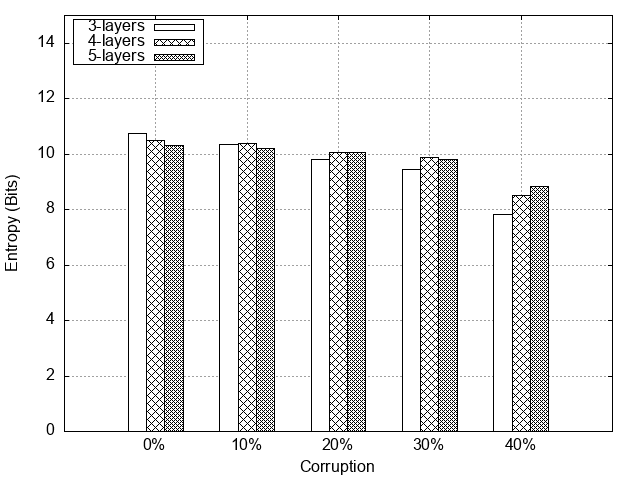
\includegraphics[height=8cm]{figures/mixim/4.png}
    \caption{Impact of Corrupted Mixes on Entropy}
    \label{fig:corrupted-mixes}
 \end{figure}

Assuredly, Figure \ref{fig:corrupted-mixes} depicts rigid results. There is a
steady decrease in anonymity each time we increase the fraction of corrupt
nodes. Moreover, it is interesting to observe that for 0\% and 10\% of
corruption, the three-layer scheme provides better anonymity, while this is not
true for 20\%, 30\% and 40\% of corruption. Instead, we notice that the higher
the corruption fraction, the lower the entropy is for the three-layer and
four-layer Stratified Mixnet. In contrast, the entropy of a five-layer design
seems to perform better. Intuitively, this is reasonable because a network with
more layers provides the possibility of having less interference by an
adversary. On the other side, a network with fewer layers but more adversarial
mixes, implies a greater possibility of maliciously influencing the communication
between mixes.

Ultimately, considering the effect of the number of layers on the network's
anonymity according to \cite{ben2021mixim}, and the results of our experiment in
Figure \ref{fig:corrupted-mixes}, we deduce that it is challenging to design a
Mixnet. In the first place, we observe that increasing the number of layers does
not much contribute to the anonymity, while introducing corrupt relays appears to
make more extensive networks necessary. Nevertheless, augmenting a Mixnet
implies computational and hardware expenses. It is beyond question that there
are some apparent tradeoffs between anonymity and scalability when adversaries
emerge.

\chapter{Exteding Current Research Using Simulator}
Chapter 5 discusses our main contribution to the Mixnets field, towards the
simulation and evaluation of arbitrarily formed Stratified networks.
Particularly, we assumed that a Stratified Mix Network might have imbalanced
layers due to crashing Mixes. Within the context of this chapter, we study two
different types of imbalanced Mixnets, which are (a) dynamically imbalanced and
(b) statically imbalanced. Additionally, we examine the impact on anonymity
caused by increasing the number of Mixes per layer. Lastly, any experiments in
this chapter operated on our modified version of Piotrowska's
Simulator\cite{simulator}.

\section{Stratified Networks with Increasing Number of Mixes}

Guirat et al.\cite{ben2021mixim} in 2021 investigated the topic of increasing the
number of layers in a Stratified network. In this section of Chapter 5, we
experiment with the number of Mixes per layer regarding Stratified networks.

Our experimental setup is relatively straightforward. We are using a Stratified
topology and the Continous mixing technique, with an average mixing delay of 0.1
seconds. Also, we are running many iterations of the experiment using a
different number of Mixes per layer. Intuitively, we expect designs with more
Mixes to yield worse anonymity. We justify our supposition, assuming that each
Mix will eventually receive less traffic. It is a matter of fact that less
traffic implies a smaller anonymity set; hence, a global adversary might be able
to identify message senders and receivers smoothly. Still, assuming that we are
using the Continous mixing technique, which has a memory-less property, the
network's entropy should fluctuate in a tight range.

\begin{figure}[h!]
    \centering
    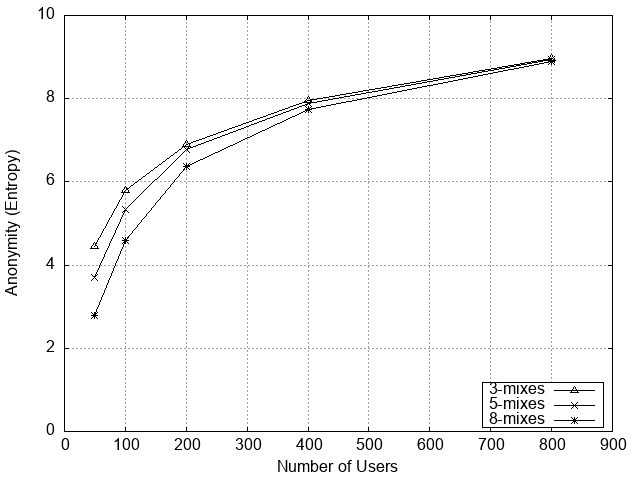
\includegraphics[height=8cm]{figures/simulator_extentions/compare_layer_size.png}
    \caption{Effect of Increasing the Number of Mixes per Layer}
    \label{fig:stratified-incresing-number-of-mixes}
\end{figure}    

Observing Figure \ref{fig:stratified-incresing-number-of-mixes} we
deduce that entropy is initially different, but as we increase the network's
user base, it converges. Potentially, we can declare that the three
interpolations are logarithmic-like for a low number of users. Nonetheless, we
are not sure if entropy diverges for a more extensive user base. Also, we notice
that netowrks with more Mixes in each layer have lower entropy for 10 to 400
users. This is reasonable because, as mentioned earlier, less traffic is routed
through mixes. Regarding the increased number of users, it is evident that
larger user bases yield better anonymity overall.


\section{Dynamically Imbalanced Stratified Network}
The notion of a dynamically imbalanced Stratified network, revolves around the
idea of having random Mixes crashing arbitrarily through different message
transmission rounds. Our goal is to make each Mix crash according to a given
probability. Mainly, we extended Simulator to handle this feature by tossing a
coin. In other words, before we sample a random route for a potential message,
we call a function producing a Real number between 0 and 1. A value less than
0.2 implies that a Mix crashes successfully, with a probability of 20\%. Also,
in the provision of a non-live route (i.e. the subsequent layer has only
malfunctioning Mixes and, therefore, we can not determine a valid path), we
increase the message queue delay by 1 second. Our decision was natural since
there is wasted time when a Mix tries to find the next live destination.

In our experimental setup, we assumed a Stratified network with three layers
comprising ten Mixes. Also, we set the mixing techniques to Continous, with an
average delay of 0.1 seconds. Then, we ran our simulation for 20\%, 40\% and 60\%
probability of failure for each Mix, individually. 

Our initial hypotheses considered that increasing the failure probability would
decrease anonymity because a considerable amount of Mixes receive less traffic.
This hypothesis is invalidated since anonymity seems to remain persistent for
different failure probabilities. According to Figure
\ref{fig:dynamic-crash-probability}, for a 20\% crash probability, we get
slightly higher entropy, assuming 100 clients in the network. Nonetheless, once
we scale up the user base and crash probabilities, the anonymity ranges in
equivalent levels. Besides that, our initial assumption for higher latency is
false since, as we notice in Figure \ref{fig:dynamic-crash-probability}, latency
remains constant. 

\begin{figure}[h!]
    \centering
    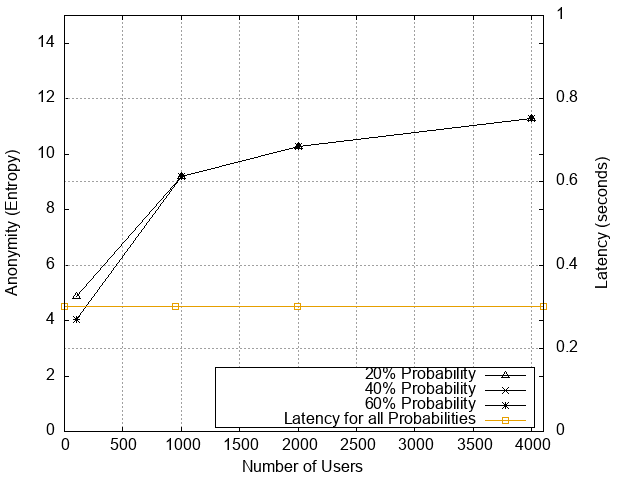
\includegraphics[height=8cm]{figures/simulator_extentions/mix_failure.png}
    \caption{Effect of Different the Crash Probabilities on Entropy}
    \label{fig:dynamic-crash-probability}
\end{figure}    


The results illustrated in the above Figure \ref{fig:dynamic-crash-probability}
are reasonable and justified through the simulation logs. In more detail,
skimming the log files, we revealed that invalid paths occur sporadically; hence,
the increased latency of a few messages does not affect the average network
latency. Moreover, anonymity is not affected because entropy fluctuations seem
to cancel out each other after simulating many messages for many users. In other
words, a route of Mixes might not appear many times in the short term, but after
sampling routes for 1000 messages, all possible paths seem to be selected an
equal number of times. Therefore, anonymity converges to a single value.

\section{Statically Imbalanced Stratified Network}

Examining the case study of a dynamically imbalanced stratified network was
fascinating. A parallel idea arose to investigate statically imbalanced
Stratified networks as well. Our perception of "static" describes a formation
where each layer has a fixed number of Mixes, yet this number is different. In
particular, we seek to study the effect on anonymity when deploying more or
fewer Mixes on the first, middle and last layer of a Stratified Mixnet. This
concept seems to be more realistic than dynamically imbalanced networks since,
when a portion of the network is down, it can be for quite some time. Hence,
statically imbalanced Mixnets might be formed for short time frames.


Our experimental setup comprises a three-layer Stratified topology enabling
Continous mixing with an average delay of 0.1 seconds. We also employ coverer
traffic of 1:1 ratio. Initially, we assess the impact on anonymity based on a
variable number of Mixes in the middle layer, testing one, two, and three
Mixes setups. Next, we repeat the same trial starting with 1 Mix and steadily
increase this number to 3 Mixes per layer for the first and last layer,
respectively.

\begin{figure}[h!]
    \centering
    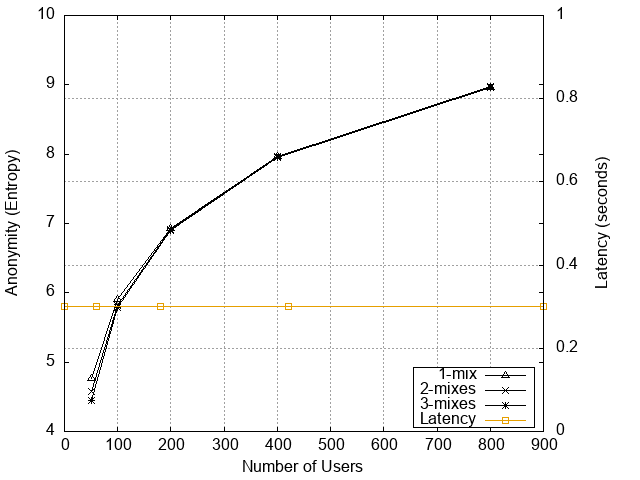
\includegraphics[height=8cm]{figures/simulator_extentions/first_layer_variable.png}
    \caption{need to add caption}
    \label{fig:first-layer-variable}
\end{figure} 

\begin{figure}[h!]
    \centering
    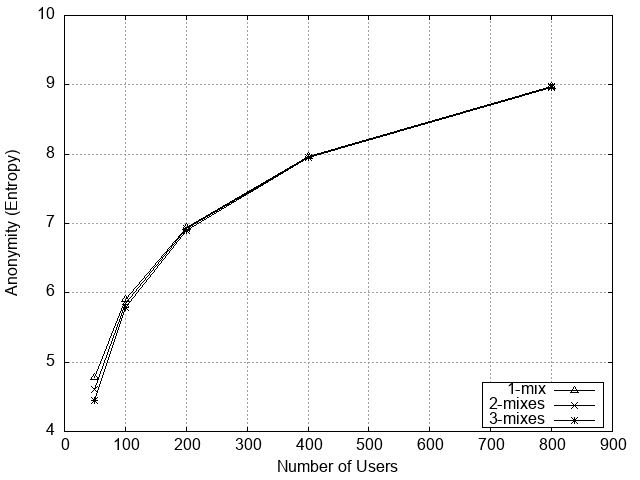
\includegraphics[height=8cm]{figures/simulator_extentions/last_layer_variable.png}
    \caption{need to add caption}
    \label{fig:last-layer-variable}
\end{figure} 

\begin{figure}[h!]
    \centering
    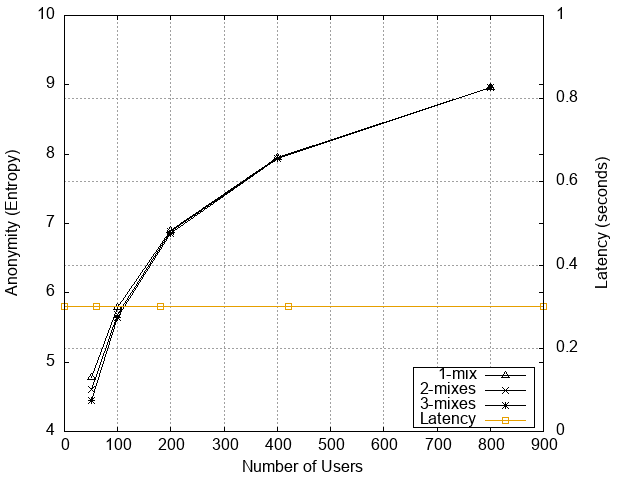
\includegraphics[height=8cm]{figures/simulator_extentions/middle_layer_variable.png}
    \caption{need to add caption}
    \label{fig:middle-layer-variable}
\end{figure} 

According to our analysis in Figures \ref{fig:first-layer-variable},
\ref{fig:last-layer-variable}, and \ref{fig:middle-layer-variable},  increasing
the number of Mixes per layer, regardless of the layer position, impacts anonymity
likewise. This is caused because all mixes repeat the same process in all layers
and traffic flows continuously from senders to Mixes and from Mixes to
recipients. Nonetheless, something different occurs assuming a smaller user
base. Notably, a three Mix per layer configuration yields slightly higher entropy
compared to two Mix layers. Likewise, a two Mix per layer network has narrowly
taller entropy than a one Mix per layer design. The results of this Figure are
credible since, by definition, routing more traffic into a Mix results in better
anonymity.

Finally, we observe latency at a constant level of 0.3. The exact value was
reported in the previous section of Chapter 5, where we simulated a dynamically
imbalanced network. This was expected since latency, as realised earlier, is not
mainly affected in network designs utilising the Continous mixing technique. 

\chapter{Conclusion}

Mix Networks provide anonymous communication against global adversaries
passively eavesdropping on network transmissions. Mixnets designs might vary
according to their topological structure, mixing algorithms and other parameters
such as cover/decoy traffic generation. Researchers developed two event-driven
simulators to assess different network designs in terms of performance and
anonymity.

Within the context of this MSc dissertation project, we report on the existing
simulators\cite{simulator,mixim} - Simulator and MiXiM - shedding light on which one should be
trusted and further developed. To bring conclusiveness to this matter, we
performed a qualitative and quantitative analysis. Mainly, we found out that
MiXiM furnishes a plethora of simulation features compared to Simulator.
Nonetheless, our study highlighted that we could not trust MiXiM since many
unrealised functions exist in the codebase. On the other hand, Simulator offers
a limited number of features, yet it is functional, generating justifiable
results. In addition, we crafted a baseline simulation scenario to test the
performance of both projects. MiXiM baseline simulations remain incomplete due
to runtime crashes. Regarding Simulator, we observe poor performance and
extended execution timeframes when increasing the number of users in a network.
Particularly, a large user base requires immense amounts of RAM (4000 users
mandate roughly 16GB of RAM).

Further, we conducted a short replication study attempting to validate previous
research\cite{piotrowska2021studying,ben2021mixim} and reason about their
results. We managed to partially replicate experiments because of hardware
limitations. As mentioned in Chapter 4, our environment's RAM was caped to 16GB.
However, our analysis revealed that, indeed anonymity of a Mixnet can be
affected by the network's topology, mixing technique and the generation of
cover/decoy traffic. Notably, a Cascade network might achieve greater anonymity
than a Multi-Cascade and a Stratified network. Also, Continous mixing yields low
latency overheads and increased anonymity due to their memory-less property.
Another intriguing highlight is that a large network user base positively
impacts its anonymity. Also, cover traffic and mixing delay are vital for
networks with small userbases as they keep anonymity to acceptable levels.
Furthermore, it is worth mentioning that in the presence of corrupted relays,
assuming a Stratified network, the anonymity decreases. 

The last contribution of our project is the investigation of dynamically and
statically imbalanced Stratified Mix Networks. As of writing this dissertation,
we are unaware of similar work in this field; hence, our research on imbalanced
networks can provide valuable insights. A dynamically imbalanced network assumes
that each Mix fails with a certain probability on each transmission round.
Anonymity and latency on such networks are not affected since after sending and
receiving numerous messages; the traffic passed through all Mixes converges,
cancelling temporal anonymity issues. On the other hand, statically imbalanced
networks consider that a layer might have more or less Mixes for longer
timeframes. Notably, we found out that the number of Mixes per layer does not
affect anonymity, especially on networks with large user bases. However, for a
limited number of users, we observed a negligible difference. Deploying fewer
Mixes, regardless of the layer, will equally favour and improve anonymity.
Finally, static and dynamic imbalanced networks' latency is low, considering the
tested Stratifed topology and Continous mixing.

In the future, we suggest exploring imbalanced Stratified Mix Networks further.
Particularly, it is worth experimenting with all mixing techniques since
threshold and timed Mixes might behave differently in an imbalanced network.
Besides that, we can adopt the dynamically imbalanced concept for Cascade and
Multi-Cascade topologies. Essentially, in Cascade networks, each Mix is a
potential point of failure. Therefore,  simulating imbalanced Cascades will
allow us to evaluate the actual overhead in latency and anonymity when a Mix
frankly goes down. To frame all of our recommendations, we propose the
development of an efficient and modular event-driven simulator, which will
support all types of topologies, mixing techniques and cover traffic
functionalities. In addition, as reported in the literature
\cite{KatzMixnet,chaum1981untraceable}, there are several methods to encrypt
messages (e.g Sphinx crpytography) flowing through Mixes. The new simulator
should allow users to explicitly define any delays that occur due to encryption
and decryption of messages. Further, a new simulator should be developed
carefully to use a few computational resources. For this reason, we propose
using Go language, a statically typed compiled language similar to C but with a
low memory footprint.

To conclude, it is essential to highlight that Mix Networks enable people to form
liberal societies where respect for privacy and anonymity prevails. Certainly,
current research provides robust knowledge on this topic. In my opinion, we need
to practically develop more applications that will benefit from using an
underline Mixnet. Finally, there is always room for improvement.

\bibliographystyle{plain}
\bibliography{mybibfile}


% You may delete everything from \appendix up to \end{document} if you don't need it.
\appendix

\chapter{Sample Configuration Files}

\section{Simulator Configuration File}
\label{appendix:a1}

\begin{lstlisting}[language=json,firstnumber=1]
{
    "experiment_id": "Simulation Stratified",
    "logging":  {
        "enabled": true,
        "dir": "logs",
        "client_log": "client_log.json",
        "mix_log": "mix_log.json"
    },
    "phases":   {
        "burnin": 100,
        "execution": 500,
        "cooldown": 2000
    },
    "network": {
        "topology" : "stratified",
        "cascade" : {
          "cascade_len": 3,
          "num_gateways": 0},
        "stratified" : {
          "layers": 3,
          "layer_size": 3,
          "num_gateways": 0
        },
        "multi_cascade" : {
          "cascade_len" : 3,
          "num_cascades" : 2
        },
        "p2p" : {
          "path_length" : 3
        }
    },
    "packet": {
        "packet_size": 0
    },
    "message": {
        "min_msg_size": 2,
        "max_msg_size": 2
    },
    "mixnodes": {
		"avg_delay": 0.1,
        "batch": false,
        "batch_size" : 1000,
		"AQM":false
    },
    "clients": {
        "number":100,
        "sim_add_buffer": 1.0,
        "rate_sending": 1.0,
        "rate_ack": 0.5,
        "cover_traffic":false,
        "cover_traffic_rate":1.0,
        "ACK":false,
        "retransmit":false,
        "dummies_acks":false,
        "max_retransmissions":5
    },
    "misc": {
        "id_len": 32,
        "num_target_packets": 1000
    }
}
\end{lstlisting}

\section{MiXiM Configuration File}
\label{appendix:a2}

\begin{lstlisting}[language=json,firstnumber=1]
[DEFAULT]
n_clients= 100
lambda_c = 1

[TOPOLOGY]
#Topology can take stratified, cascade, free route
type = stratified
fully_connected = True
routing = source
E2E = 1
n_layers = 1
#If stratified
l_mixes_per_layer = 10
#If Cascades
n_cascades = 3
[MIXING]
#mix_type takes poisson, time, or pool
mix_type = poisson
mu = 1
timeout = 2
threshold = 100
flush_percent = 0.1
[DUMMIES]
client_dummies = False
rate_client_dummies = 1
link_based_dummies = True
multiple_hop_dummies = False
rate_mix_dummies = 1
[NODES_SELETION]
#Probability over nodes selection: uniform, specific
probability = Uniform
#if specific
    #if topology = stratified
w_mix_l1 = [0.5]
w_mix_l2 = [0.3]
w_mix_l3 = [0.1]
    #if topology = cascade
w_cascades = [0.8, 0.1, 0.1]

[THREATMODEL]
corrupt_mixes = 0
balanced_corruption = True    
\end{lstlisting}


\chapter{cProfile Execution Trees}

\section{Simulator Execution Tree}
\label{appendix:b1}
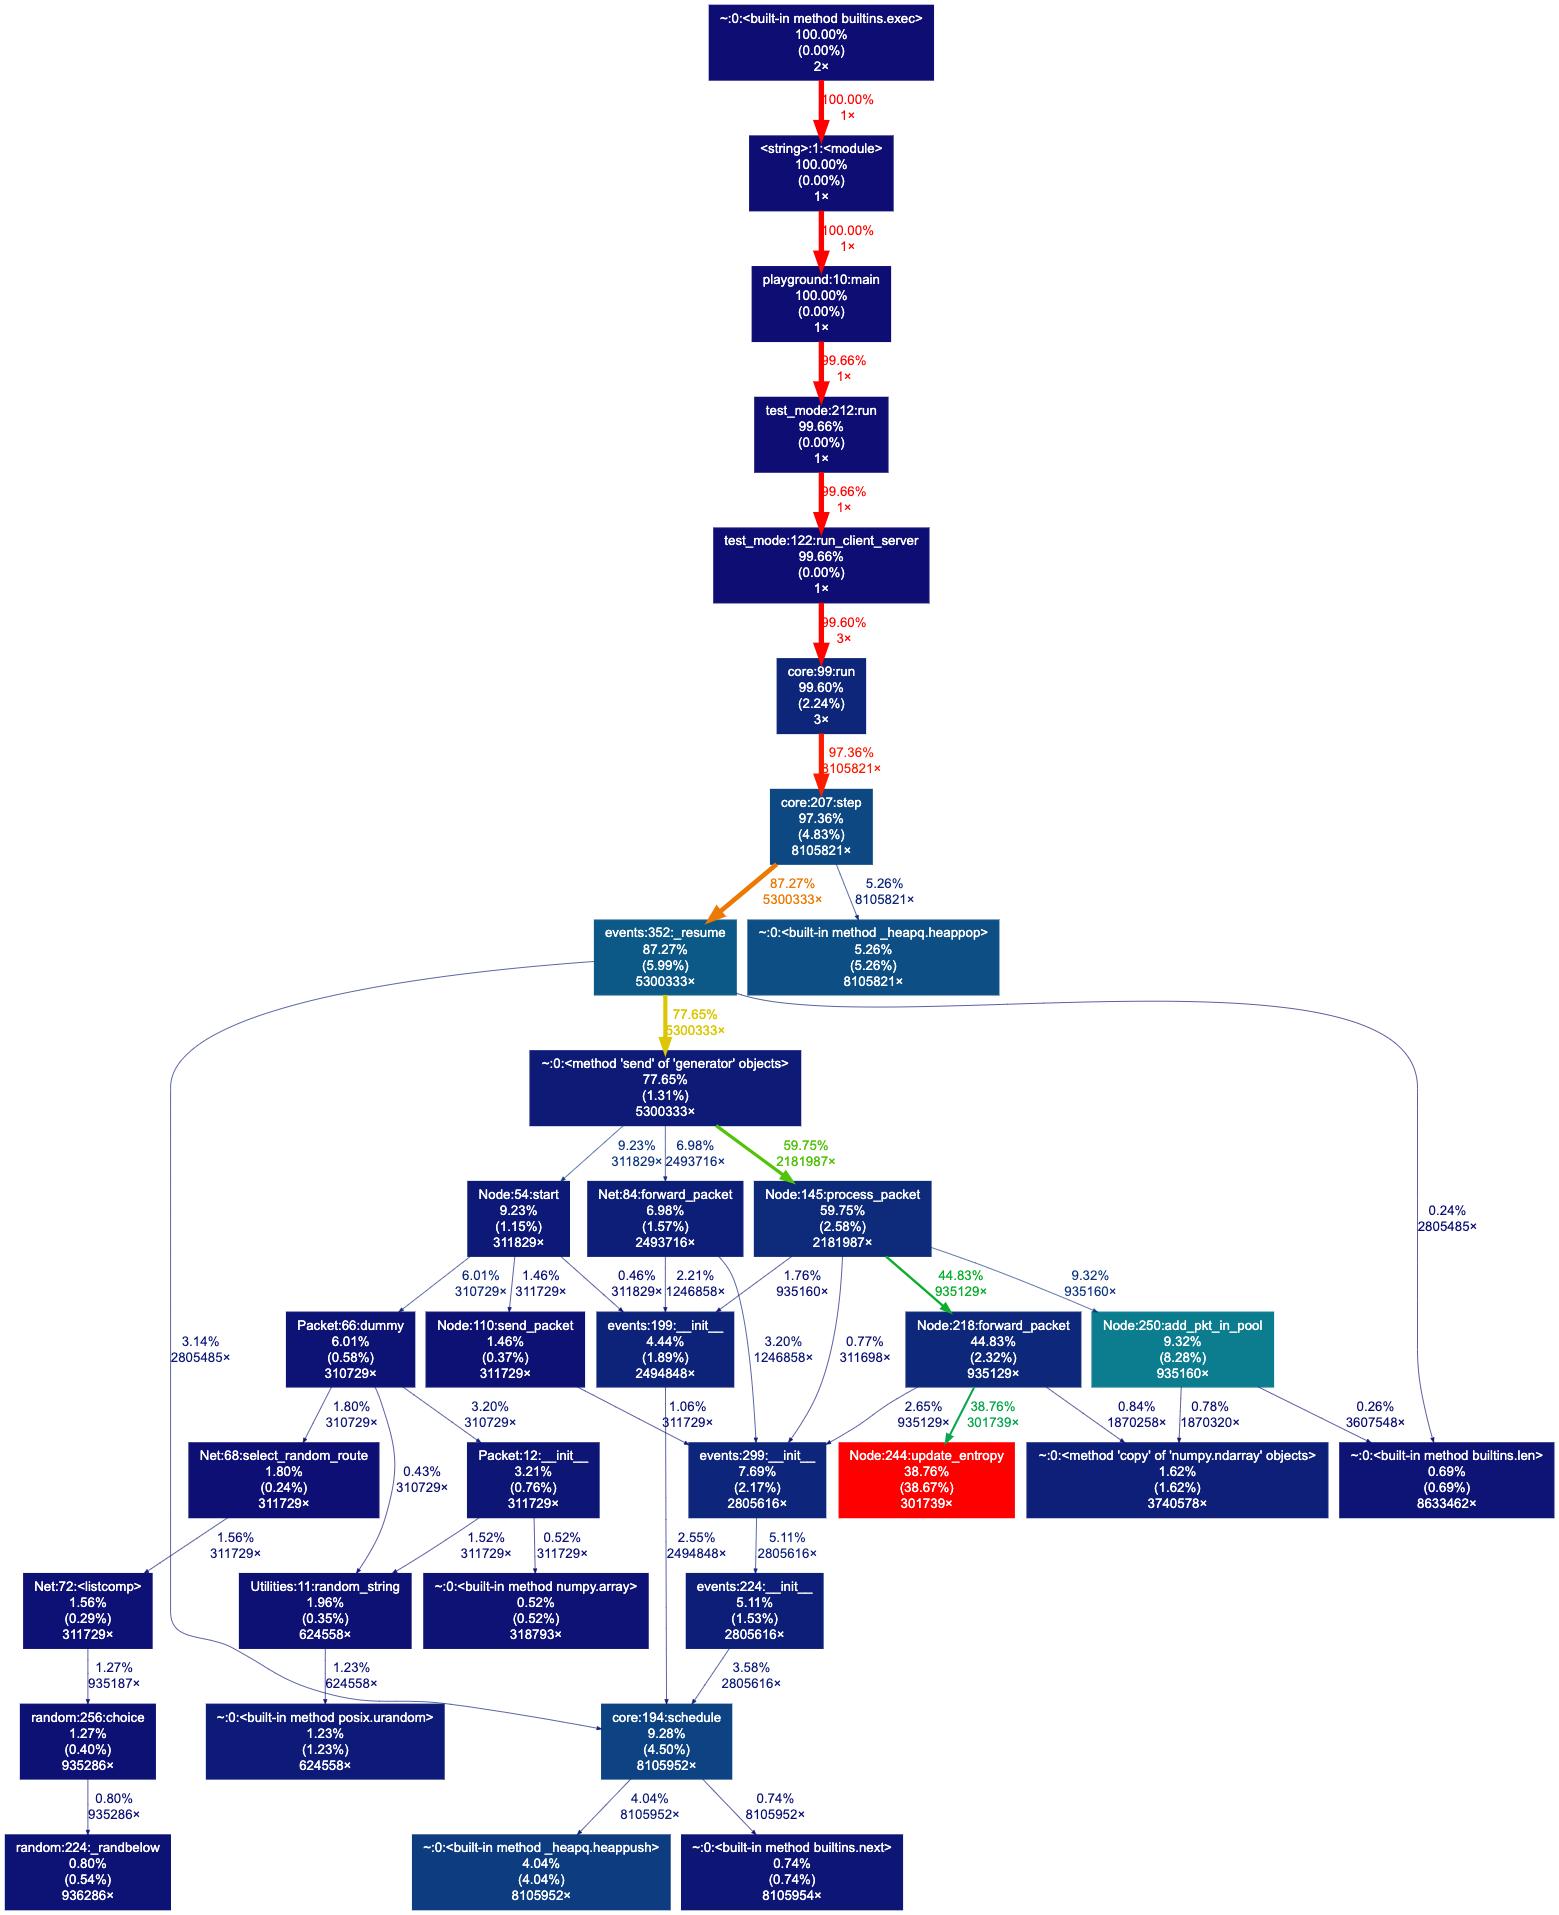
\includegraphics[width=\textwidth]{images/cprofile_simulator.png}

\section{MiXiM Execution Tree}
\label{appendix:b2}
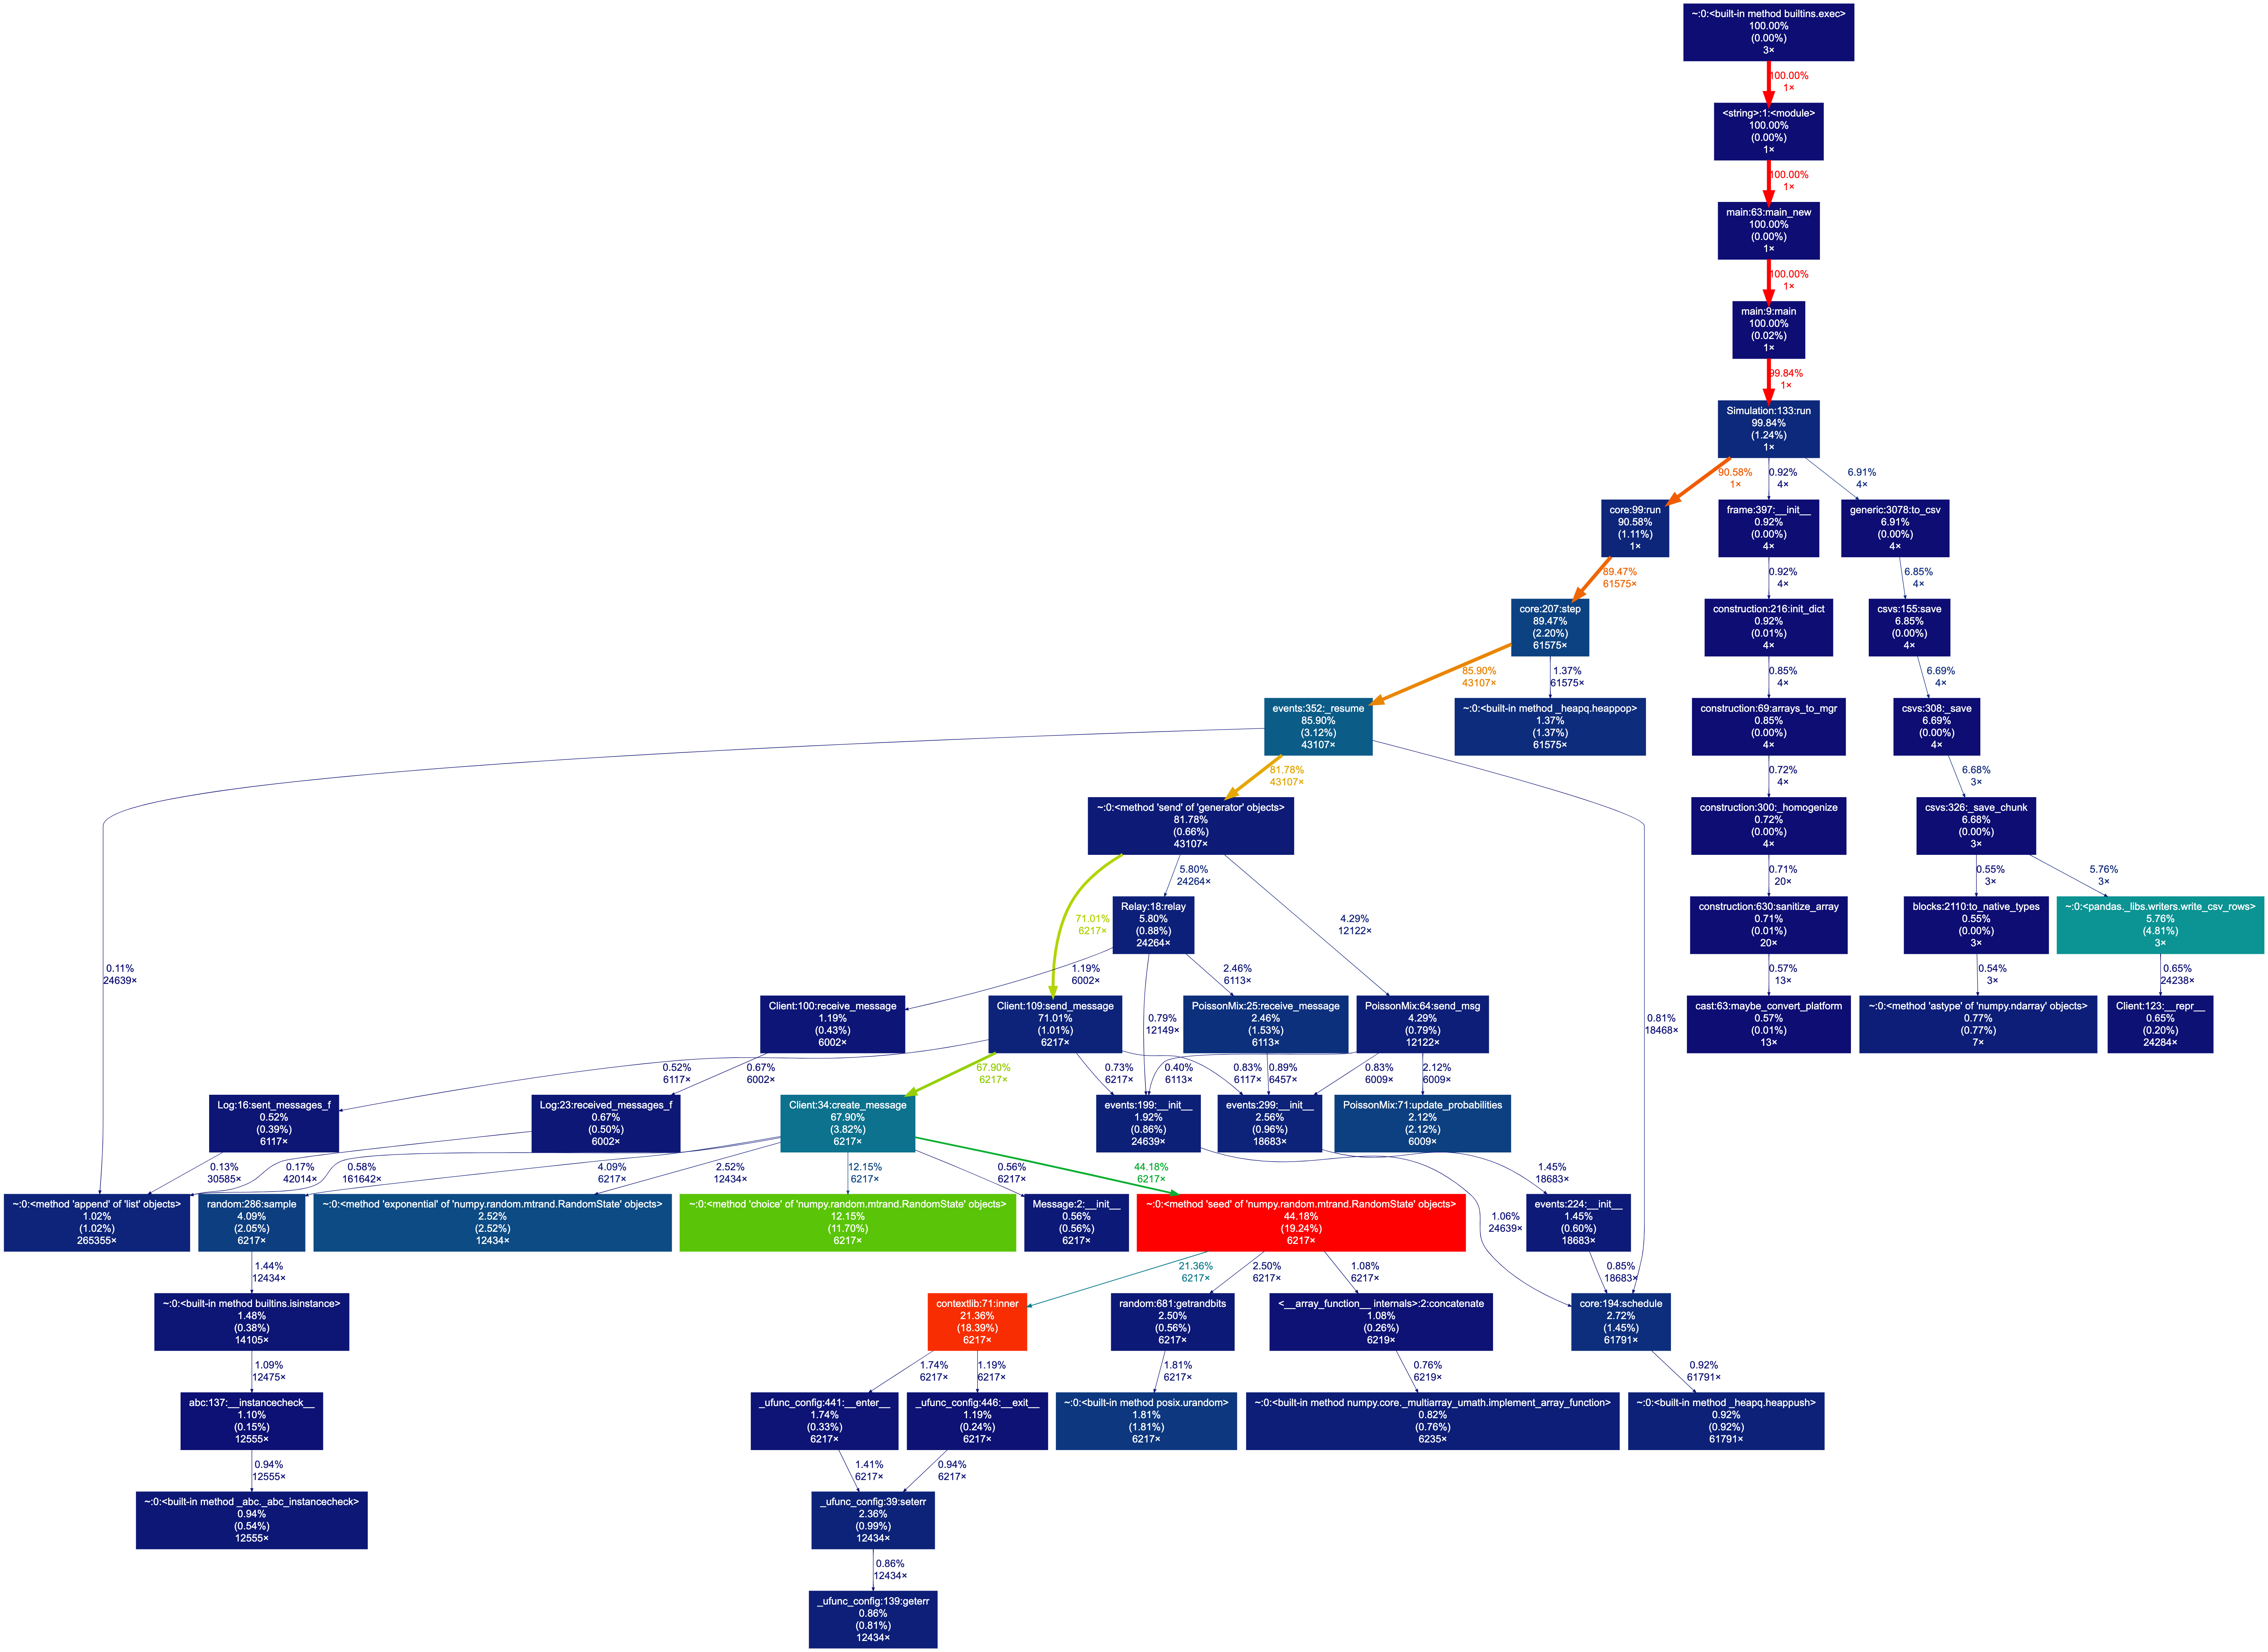
\includegraphics[width=\textwidth]{images/cprofile_mixim.png}


\end{document}
